%
% parita-msc.tex -- main file for my thesis
%
\documentclass[12pt]{report}
\usepackage{caption}
\setcounter{secnumdepth}{5}
\setcounter{tocdepth}{2}
\usepackage{setspace}
\usepackage{graphicx}
\usepackage{adjustbox}
\usepackage{subcaption}
\usepackage{amsmath}
\usepackage{textcomp}
\usepackage{ragged2e}
\usepackage{indentfirst}
\usepackage{floatrow}
\usepackage{float}
\usepackage[table]{xcolor}
\usepackage{multicol}
\usepackage{array,multirow}
\usepackage[margin=3cm]{geometry}
\usepackage[autostyle]{csquotes}
\usepackage[table]{xcolor}
\usepackage[T1]{fontenc}
\usepackage{multicol}
\usepackage{listings}
\usepackage[toc,page]{appendix}
\usepackage{adjustbox,lipsum}
\usepackage{enumitem}
\usepackage{amssymb}
\usepackage{fancyhdr}
\usepackage{dirtytalk}
\usepackage{listings}
\usepackage{url}
\def\UrlBreaks{\do\/\do-}
\usepackage{breakurl}
\usepackage[breaklinks]{hyperref}

\usepackage{acro}
\acsetup{
	list-style=tabular, 
	only-used=true, 
	sort=true,
	page-style=plain, 
	pages=first
}
%!TEX root = parita-msc.tex
\DeclareAcronym{uri}{
  short = URI ,
  long  = Uniform Resource Identifiers ,
  class = abbrev
}
\DeclareAcronym{http}{
  short = HTTP ,
  long  = Hyper Text Transfer Protocol ,
  class = abbrev
}
\DeclareAcronym{https}{
  short = HTTPS ,
  long  = Hypertext Transfer Protocol Secure ,
  class = abbrev
}
\DeclareAcronym{ssl}{
  short = SSL ,
  long  = Secure Socket Layer ,
  class = abbrev
}
\DeclareAcronym{sparql}{
  short = SPARQL ,
  long  = Simple Protocol and RDF Query Language ,
  class = abbrev
}
\DeclareAcronym{rdf}{
  short = RDF ,
  long  = Resource Description Framework  ,
  class = abbrev
}
\DeclareAcronym{www}{
  short = WWW ,
  long  = World Wide Web  ,
  class = abbrev
}
\DeclareAcronym{w3c}{
  short = W3C ,
  long  = World Wide Web Consortium ,
  class = abbrev
}
\DeclareAcronym{html}{
  short = HTML ,
  long  = Hyper Text Markup Language ,
  class = abbrev
}
\DeclareAcronym{url}{
  short = URL ,
  long  = Uniform Resource Location ,
  class = abbrev
}
\DeclareAcronym{urn}{
  short = URN ,
  long  = Uniform Resource Name ,
  class = abbrev
}
\DeclareAcronym{xml}{
  short = XML ,
  long  = eXtensible Markup Language ,
  class = abbrev
}
\DeclareAcronym{rdfs}{
  short = RDFS ,
  long  = Resource Description Framework Schema ,
  class = abbrev
}
\DeclareAcronym{lod}{
  short = LOD ,
  long  = Linked Open Data ,
  class = abbrev
}
\DeclareAcronym{lov}{
  short = LOV ,
  long  = Linked Open Vocabulary ,
  class = abbrev
}
\DeclareAcronym{sql}{
  short = SQL ,
  long  = Structured Query Language ,
  class = abbrev
}
\DeclareAcronym{csv}{
  short = CSV ,
  long  = Comma Separated Values ,
  class = abbrev
}
\DeclareAcronym{owl}{
  short = OWL ,
  long  = Web Ontology Language ,
  class = abbrev
}
\DeclareAcronym{tsv}{
  short = TSV ,
  long  = Tab Separated Values ,
  class = abbrev
}
\DeclareAcronym{gdpr}{
  short = GDPR ,
  long  = General Data Protection Regulation ,
  class = abbrev
}
% European Council for Nuclear Research
\DeclareAcronym{cern}{
  short = CERN ,
  long  = Conseil Européen pour la Recherche Nucléaire ,
  class = abbrev
}
\DeclareAcronym{er}{
  short = ER ,
  long  = Entity Relationship ,
  class = abbrev
}
\DeclareAcronym{turtle}{
  short = Turtle ,
  long  =  Terse RDF Triple Language ,
  class = abbrev
}
\DeclareAcronym{n3}{
  short = N3 ,
  long  =  Notation3 ,
  class = abbrev
}
\DeclareAcronym{vowl}{
  short = VOWL ,
  long  =  Visual Web Ontology Language ,
  class = abbrev
}
\DeclareAcronym{svg}{
  short = SVG ,
  long  =  Scalable Vector Graphics ,
  class = abbrev
}
\DeclareAcronym{json}{
  short = JSON ,
  long  =  JavaScript Object Notation ,
  class = abbrev
}
\DeclareAcronym{ide}{
  short = IDE ,
  long  =  Integrated Development Environment ,
  class = abbrev
}
\DeclareAcronym{png}{
  short = PNG ,
  long  =  Portable Network Graphics ,
  class = abbrev
}
\DeclareAcronym{jpeg}{
  short = JPEG ,
  long  =  Joint Photographic Experts Group,
  class = abbrev
}
\DeclareAcronym{gif}{
  short = GIF ,
  long  =  Graphics Interchange Format ,
  class = abbrev
}
\DeclareAcronym{api}{
  short = API ,
  long  =  Application Programming Interface ,
  class = abbrev
}
\DeclareAcronym{iri}{
  short = IRI ,
  long  =  Internationalized Resource Identifier ,
  class = abbrev
}
\DeclareAcronym{iso}{
  short = ISO ,
  long  =  International Organization for Standardization ,
  class = abbrev
}
\DeclareAcronym{gui}{
  short = GUI ,
  long  =  Graphical User Interface ,
  class = abbrev
}
\DeclareAcronym{grel}{
  short = GREL ,
  long  =  Google Refine Expression Language ,
  class = abbrev
}
\DeclareAcronym{dl}{
  short = DL ,
  long  =  Description Logics ,
  class = abbrev
}
\DeclareAcronym{obda}{
  short = OBDA ,
  long  =  Ontology-Based Data Access ,
  class = abbrev
}


%
% added following 3 lines to define "definition" -- see what you think
\usepackage{amsthm}
\theoremstyle{definition}
\newtheorem{definition}{Definition}[section]
% added above 3 lines
%
\newcommand{\myparagraph}[1]{\paragraph{#1}\mbox{}\\}
%\tracingassigns=1\tracinggroups=1\tracingall
\begin{document}
\begin{titlepage}
    \begin{center}
    \begin{doublespace}
        \vspace*{3cm}

        \large
%         A model for creation of Vocabularies in Ontology for a Survey 
%	   Designing linked open vocabularies for Linked Data Applications
%	   Creating a Linked Data Application for Surveys
%	   Defining new linked open vocabularies for Student Feedback Application
			%Creating a Linked Data Application
			%Usability Issues in Creating a Linked Data Application
			%A Guide for the Development and Evaluation of Adequacy of a Linked Open Vocabulary for a Feedback Survey
			Development of a Linked Open Vocabulary for a Feedback Survey

        \vspace{1cm}

        \large
        A Thesis\\
        Submitted to the Faculty of Graduate Studies and Research\\
        In Partial Fulfillment of the Requirements\\
        For the Degree of\\
        Master of Science\\
        in Computer Science\\
        University of Regina\\

        \vspace{0.8cm}

        \normalsize
        By\\
        Parita Dipakkumar Amin\\
        Regina, Saskatchewan\\
        August, 2022\\

        \vspace{0.8cm}
        \textcopyright \hspace*{0.2cm} Copyright 2022: Parita Amin%$\sim$
    \end{doublespace}
    \end{center}
\end{titlepage}

\newpage
\pagenumbering{roman}
\addcontentsline{toc}{chapter}{Abstract}
%!TEX root = parita-msc.tex

\begin{doublespace}
\begin{center}
\textbf{Abstract}
\end{center}

The \ac{www}, as defined by the \ac{w3c}
at {\tt https://www.w3.org/WWW/}, 
is ``the universe of network-accessible information, 
the embodiment of human knowledge''. 
With development 
%in study and research 
over the years, 
the global web of linked documents has become the global web of linked data, 
which is popularly known as the Semantic Web.
%\footnote{https://www.w3.org/standards/semanticweb/}.

The Semantic Web is now an established topic of research but there remain many unanswered questions.
\ac{lod}, as the highest standard for linked data, is a worthy goal for researchers and data providers
who seek to contribute to the development of the Semantic Web.
Data that are linked and open facilitate discovery and reuse.
Likewise, vocabularies used to describe the semantic relationships amongst data
that are linked and open facilitate discovery and reuse.
%, to become parts of new data
Yet, it is not always a straightforward matter to take data that may be somehow accessible on a webpage written in \ac{html} and publish it as \ac{lod}.
%and it has not been completely explored yet. 
%In addition to this, open source gives comparatively more development opportunities to all the researchers and developers to discover, build and reuse existing data. 
%The linked open data on the web is designed using linked open vocabularies.
%This thesis describes a model of creating new linked open vocabularies or reusing the existing ones. 
%The thesis also includes the 
Many complimentary technologies are used in handling \ac{lod} on the web,
particularly the \ac{rdf}, the \ac{owl}, and the \ac{sparql}. 
%All these technologies have their own distinct purposes which are further discussed in the thesis.
 
 \marginpar{last paragraph news some attention -- presently commented out}
%Vandenbussche et al.~\cite{pierre2017vocabularies} in 2017 stated 
%that \say{the \ac{lov} initiative gathers and makes visible indicators such as the interconnections between vocabularies and each vocabulary's version history, 
%along with past and current editor (individual or organization)}. 
%This thesis work is in contribution to the same initiative and to Berners-Lee's vision. 
%As a part of this research, 
%a model for survey ontology was developed in order to assist the study which is described in detail in Chapter~\ref{chap:ontology}. 
%There are multiple opportunities for future work like
%creation of new vocabularies required for other types of surveys and more research work.

\end{doublespace}

\newpage
\addcontentsline{toc}{chapter}{Acknowledgments}
%!TEX root = parita-msc.tex

\begin{doublespace}
\begin{center}
\textbf{Acknowledgements}
\end{center}

I would like to take an opportunity to thank all the people who have supported me during my research period in some or the other way.

I would like to express my soulful gratitude to my supervisor Dr. Daryl H. Hepting for his valuable time, guidance, suggestions and comments throughout the course of the research. He was always open to all my questions and queries related to my research work as well as while writing 
%DHH added "this"
this
thesis. 
He provided me with the space required to make this study as my own work, at the same time he made sure that I am leading on the right path by giving constant feedback and suggestions whenever I was lost or stuck. I would also like to thank the Department of Computer Science and Faculty of Graduate Studies and Research for their academic as well as administrative support as and when required.

Lastly, I am grateful to my parents for always being there for me regardless of the distance and time-difference between the two different parts of the world. This would have been next to impossible for me if not for them. I would like to specially thank my brother Shivam for being the family here and for encouraging and motivating me during the times I was low. My special thanks to all my friends for all their support.

\end{doublespace}


\newpage
\addcontentsline{toc}{chapter}{Post-Defense Acknowledgments}
%!TEX root = parita-msc.tex

\begin{doublespace}
\begin{center}
\textbf{Post-Defense Acknowledgements}
\end{center}


\end{doublespace}


\renewcommand{\contentsname}{Table of Contents}
\tableofcontents
\cleardoublepage

\addcontentsline{toc}{chapter}{\listfigurename}
\listoffigures
\cleardoublepage

\addcontentsline{toc}{chapter}{\listtablename}
\listoftables
\cleardoublepage

\addcontentsline{toc}{chapter}{List of Abbreviations}
%%\begin{doublespace}
\printacronyms[include-classes=abbrev,name={List of Abbreviations},heading={chapter*}]
%%\end{doublespace}
\cleardoublepage

\pagenumbering{arabic}
%!TEX root = parita-msc.tex

\chapter{Introduction}
\label{chap:intro}
\begin{doublespace}

Tim Berners-Lee is 
%considered as 
the father of the \ac{www}.
He wrote
\emph{Information Management: A Proposal}\footnote{{\tt https://www.w3.org/History/1989/proposal.html}, dated March 1989, May 1990} in 1989 and 1990
to present the need for a \say{global hypertext system} at the \ac{cern}.
In his conclusion to that document, he wrote:
\blockquote{\enquote{we should work toward a universal linked information system, 
in which generality and portability are more important than fancy graphics techniques and complex extra facilities. 
The aim would be to allow a place to be found for any information or reference which one felt was important and a way of finding it afterward. 
The result should be sufficiently attractive to use, 
that is, 
the information contained would grow past a critical threshold 
so that the usefulness of the scheme would, 
in turn, 
encourage its increased use.}}

In the more than 30 years that have followed that initial proposal,
a great deal of progress towards Berners-Lee's vision has been realized.
The original \say{web of documents} is becoming the \say{web of data} or the
\say{semantic web}. 
Is this next web sufficiently attractive to use?
This thesis will examine this question in the context of an example.

\section{Motivation}

In his teaching practise, 
my supervisor collects feedback from students in his classes each semester 
and makes the responses available on his 
website\footnote{\tt http://www2.cs.uregina.ca/~hepting/teaching/evaluation.html}.
Typically, student responses were collected on paper and then entered manually into
computer-readable form.
This was not done during the {COVID}-19 pandemic.

Although it is valuable to have this data available on the web,
it is not published as \ac{lod}.
The motivation for the research presented here was to examine the
process by which existing data can be published as \ac{lod} and
to consider whether that process is ``sufficiently attractive to use''.
%. The data has been
%uses a survey to collect feedback from students taking his classes each semester. 
%He makes the responses available on his website. The responses are collected on paper and then entered manually and stored in tabular form. Dr. Hepting and I were intrigued to know if it is possible to have the data available as linked open data. While researching for the ontology vocabularies that I can reuse for our application, I got to know there exists negligible research and development for the vocabularies that can be used to describe a \say{survey} ontology. This motivated me more to try to describe linked open data vocabularies for a feedback survey.

%Working further on the vision of Berners-Lee for the current web, this thesis focuses on the aim of providing important information that can be useful for someone working in the same direction.

%Data science~\cite{dhar2013} is a multifaceted field of computer science in which knowledge is extracted from various structured and unstructured data. Different scientific methods, algorithms, techniques, processes, and systems are used for data extractions. Data science is a vast field that covers numerous other fields under its umbrella. One such field is data management. Data management, on the contrary, is the study of data storage, representation, and accessibility.
%
%Sometimes, it is important to publish structured data and link it to already available structured data on the web, which makes searching the information on the web using semantics (keywords) more efficient and easier. Publishing unstructured data does not help the searches using keywords. 

The published linked (structured) data which is available on the web can be efficiently retrieved and reused as, according to Ngomo et al.~\cite{ngomo2014introduction}, linked data is \say{a set of best practices for publishing and connecting structured data on the web}.
%\marginpar{I suggest dealing with TBL's Design Issues post (berners1996linked) as the source for this part: I have referenced it right before the principles in order to include other related references}
After the introduction of the semantic web and the four principles of linked data for publishing and connecting structured datasets on the web by Berners-Lee, the web of documents has been gradually moving towards the development of the web of data. 
With time, these principles have been accepted and considered as the standard to publish structured data on the semantic web~\cite{bizer2009emerging, bizer2011linked, bizer2008linked, heath2011linked}. 
The four principles of linked data by Berners-Lee~\cite{berners1996linked}
\label{principles} 
are as follows:

\begin{itemize}
  \item Use \ac{uri} as names for things
  \item Use \ac{http}\footnote{Both \ac{http} and \ac{https}} \ac{uri}s to look up those names
  \item Provide useful information, using the standards (\ac{rdf}\footnote{includes all the standards belonging to \ac{rdf} family}, \ac{sparql})
  \item Include links to other \ac{uri}s to discover more things
\end{itemize}

After the development of Linked Data for the semantic web, 
%\marginpar{I suggest starting with 0 stars and building up to 5 and cross-reference the 4 principles in that if you can: should it be in chapter 1 or 2?}
Berners-Lee also contributed to web engineering by introducing a 5-star rating\footnote{https://www.w3.org/2011/gld/wiki/5\_Star\_Linked\_Data} system for the rating of linked data implementations. 
In this system, using the linked data principles, the publishers of the data on the web link their data to the existing linked data to provide reference and make it available for lookup. The data on the web, according to the 5-star system, is accepted to be 5-star data if the data:

\begin{itemize}
  \item is structured (machine-readable)
  \item has open-license for access
  \item is described and linked to other data using \ac{uri}s
\end{itemize}

%Today, it is necessary to build a system where the unstructured data (data that is not yet available as linked data) can be transformed into linked data (structured) and published on the web using the Linked Data Life Cycle\footnote{https://www.w3.org/2011/gld/wiki/GLD\_Life\_cycle}. This transformation of publishing structured linked data will allow the users to carry out various functions and processes on the web, which was not possible earlier along with raising the importance, fruitfulness, and effectiveness of the datasets. 

A query\footnote{https://www.techopedia.com/definition/5736/query} is used to retrieve information from a database that consists of multiple tables. 
According to the \ac{w3c} recommendation, a semantic (web) query depicts the techniques and protocols that are \say{used to retrieve information from the web of data} using computer programs. Web (semantic) queries use the semantics and the constitution of data on the web to perform data retrieval operations. Various semantic web technologies have been developed for data retrieval on the web. \ac{sparql} is one of the semantic web technologies used for web queries, where it gathers all the data from different domains and treats all those datasets as local.
%\marginpar{talking about queries is good - foreshadow  inclusion of a query on your sample data -- in Chapter 4. Maybe do this with respect to LD Life Cycle that is tailored to this example of the feedback data: I don't necessarily understand this}

\section{Contribution}

%The application of data science in the real world, 
%till today, 
%has been limited to technology firms and industries. 
%The field is still being explored and hence, a lot of research work is going on as the focus is on the development of the technology. 
%The use of data science in day-to-day life still requires a lot of research and development work. 
%This research work is a small trial towards using the semantic web for non-computer-related tasks. There exists almost negligible work done related to the development of linked open vocabularies 
%for a survey. 
%An open-source ontology development tool, Protégé, has been used for the development of the new vocabularies. The instrument developed is an example of a set of survey vocabularies that can be described in correspondence to the design. 
%For this research, the vocabulary mentioned is for the feedback form that Dr. Hepting uses for receiving feedback from the students for each course that he teaches.

\section{Organization}

Following this introduction, the rest of the thesis is organized as follows.
Chapter 2...
Chapter 3...
Chapter 4...
Finally, Chapter 5 presents some conclusions and opportunities for future work.

%\par Standard Pizza ontology\footnote{https://protegewiki.stanford.edu/wiki/Protege4Pizzas10Minutes} is a user guide developed at Stanford University to help the users, step-by-step, in describing new vocabularies using Protégé. Protégé\footnote{https://protegewiki.stanford.edu/wiki/Main\_Page} is an open-source ontology development environment that supports the tools to build knowledge-based applications. The Protege4Pizza10Minutes has acted as a motivation to the research work described in this thesis. The thesis follows a specific methodology to build a model to describe forms for various surveys. Once the vocabulary is described, it is easier to use different ways of representation to explain the relationships among the entities as well as the properties. Some of the commonly used visualization tools are also described in the later part of the thesis. 
\end{doublespace}
%!TEX root = parita-msc.tex

\chapter{Related Work}
\label{chap:relwork}
\begin{doublespace}

This chapter includes the theoretical and conceptual information that builds the foundation for this thesis.
Broadly, this chapter covers the semantic web and linked open data from the two perspectives of technology and usability. 

%The study of semantic web and related concepts has been successful in drawing the interest of many researchers, data scientists, and web designers. But, topics like semantic web and linked data are still too wide to be discovered and explored. There are still some related areas that have not been explored yet. The topic of research here is a small attempt at one of those unexplored topics. 


\section{The Web}

The idea of the Web, as per Berners-Lee~\cite{bernersreadings}, was derived from a positive experience of a small \say{home-brew}, a personal hypertext system. This \say{home-brew} system was used to keep track of personal information on a distributed project. The Web can be used independently for multiple projects that can be later integrated with unique relationships among them using the newly shaped information to represent the new state of linked knowledge.
The web was first designed by Berners-Lee in 1989\footnote{https://www.w3.org/History/1989/proposal.html} while working at the \ac{cern}. The web, today, has advanced more, evolved, and progressed to develop multiple versions. Different versions of the Web were designed and declared as generations like Web 2.0, Web 3.0, and Web 4.0. Web 2.0 has been accepted and included for a long time now, Web 3.0 is comparatively new, whereas Web 4.0 is at the initial stage of research and application. An idea of different versions of the web can be derived from Figure~\ref{fig:2.1}.
\begin{figure}[htp]
    \centering
    
\includegraphics[width=15cm]{images/ch2/Figure1.png}
    \caption{Different Versions of the Web, according to Aghaei et al.~\cite{aghaei2012evolution}}
    \label{fig:2.1}
\end{figure}

The first version of the Web designed in 1989, as per Aghaei et al.~\cite{aghaei2012evolution}, was read-only. 
The users of the web browsers for Web 1.0 could only read the information present on the web pages. The right to modify the contents of the web page was only with the website owners. 
In 2004, Dale Dougherty at O'Reilly Media~\cite{aghaei2012evolution} formally designed an improved version of Web 1.0 and called it Web 2.0 where the users had the liberty to read as well as modify the data on the web. The web browsers for this generation of the web offered comparatively more features than Web 1.0, making the websites more efficient and engaging. Features like web designing, creation, and modification also helped Web 2.0 in the introduction of blogs, vlogs, wikis\footnote{www.wiki.org/wiki.cgi?WhatIsWiki} and social networking technologies~\cite{harris2009web}.

\section{Semantic Web}

In 2006, John Markoff~\cite{aghaei2012evolution} introduced the new read-write-execute web as Web 3.0 in New York Times. Structured datasets and the links between them are used for the successful working of Web 3.0, also known as the Semantic Web. The web pages for the semantic web can be written using \ac{html} and \ac{rdf} as it is the web of data, contrary to the web of documents, where the web pages were written using \ac{html} and the links were described using hyperlinks. In the web of data, arbitrary things can be expressed using links to represent the relationship between two entities, as shown in Figure~\ref{fig:2.2}.

\begin{figure}[htp]
    \centering
    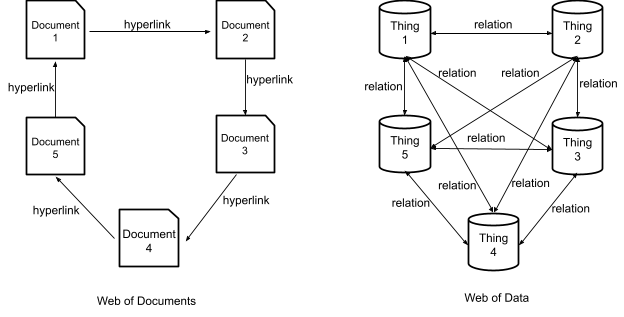
\includegraphics[width=15cm]{images/ch2/Figure2.png}
    \caption{The Web to Semantic Web, according to Aghaei et al.~\cite{aghaei2012evolution}}
    \label{fig:2.2}
\end{figure}

The latest generation of web that is still at its research and development stage is Web 4.0 which is supposed to be read-write-execute with the property of concurrency~\cite{choudhury2014}. This version of the web is intended to work with artificial intelligence to give users an exceptional quality of experience. While describing how Web 4.0 would be, Berners-Lee~\cite{bernerslee1999weaving}
stated \say{if \ac{html} and the Web made all the online documents look like one huge book, \ac{rdf}, schema, and inference languages will make all the data in the world look like one huge database}.
\subsection{The Semantic Web Stack}
\par The Semantic Web Stack
\footnote{https://en.wikipedia.org/wiki/Semantic\_Web\_Stack} is also known as Semantic Web Cake or Semantic Web Layer Cake. The stack represents the architecture of semantic web. Figure~\ref{fig:2.3}\footnote{https://www.w3.org/2001/12/semweb-fin/w3csw} shows how semantic web principles are implemented in the layers of technologies.
\begin{figure}[htp]
    \centering
    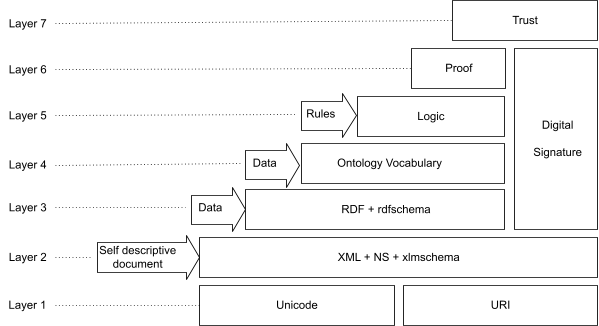
\includegraphics[width=15cm]{images/ch2/Figure3.png}
    \caption{Semantic Web Stack}
    \label{fig:2.3}
\end{figure}
\par The layers in the stack consist of different technologies. Going from the lowest level to the top level, the technologies are Unicode and \ac{uri}; \ac{xml}, NS and xmlschema; \ac{rdf} and rdfschema; Ontology vocabulary; Logic; Proof; and Trust. Digital signatures are used as security at different levels. The layers belong to three different groups, namely, self-descriptive document, data and rules.
\section{Linked Open Data}
\par According to Berners-Lee et al.~\cite{aghaei2012evolution}, \say{Semantic web is not limited to publication of data on the web; it is about making links to connect related data.} The concept of Linked Open Data\footnote{https://www.ontotext.com/knowledgehub/fundamentals/linked-data-linked-open-data/} is an amalgamation of two technologies, Linked Data and Open Data. GraphDB\footnote{https://www.ontotext.com/knowledgehub/fundamentals/linked-data-linked-open-data/} by Ontotext, an \ac{rdf} database, is an example of \ac{lod}. GraphDB promotes knowledge-discovery and efficient data-driven analytics by linking large datasets from distinct sources to Open Data.
\subsection{Linked Data}
\par The relationships shared among the data from different sources on the web are equally important as the access to the data for efficient working of the semantic web. The technique used to manage these datasets and their relationships is referred to as Linked Data. In other words, Linked Data\footnote{https://www.w3.org/wiki/LinkedData} can be termed as a set of various techniques of publishing structured data on the web. The \ac{w3c} standards and various semantic web technologies handle the distribution and engagement of the structured data across the web to aggregate the data available on the web into one huge database~\cite{bernerslee1999weaving}.
\par In 2006, Berners-Lee~\cite{bizer2009linked} framed four basic rules (mentioned in section \ref{principles}) to publish and connect the structured datasets across the web. This set of rules was termed as Linked Data principles. A brief description of these principles is as follows:
\begin{enumerate}
  \item Use \ac{uri}s as names for things:
  \par The web identifiers, the (\ac{uri}s) should be used to give unique names to all the entities (or things) on the web. \ac{uri} of an entity can be used to understand that the entity in this dataset is the same as the other entity in a disparate dataset. 
  \item Use \ac{http}\footnote{Both \ac{http} and \ac{https}} \ac{uri}s to look up for those names:
  \par The \ac{http}/\ac{https} protocols allow easy retrieval of resources. Hence, along with \ac{uri}s, either of the protocols can be used to search things (entities) easily. This promotes the publication of data on the web and its addition to the global data space.
  \item Provide useful information, using the standards (\ac{rdf}\footnote{includes all the standards belonging to \ac{rdf} family}, \ac{sparql}) to look up for a \ac{uri}:
  \par When an entity is searched using the \ac{uri} associated with it, it is beneficial to use standards like \ac{rdf} and \ac{sparql} to query the datasets. \ac{rdf} is a framework used for graphical representation of publication and distribution of data on the web, as described in detail in section~\ref{section:rdf}. On the contrary, \ac{sparql} is a query language used for retrieval and manipulation of data (in \ac{rdf} format) on the web. It also helps with the information on relationships related to the data being searched.
  \item Include links to other \ac{uri}s to discover more thing:
  \par In the semantic web, links between two entity defines the relationship using the basic entity-relationship model. Using links for \ac{uri}s of the entities promotes interconnection of the data and search of things on the web. Connecting new data to already existing entities increases the reuse and interlinking within the domain and creates a computer-understandable network.
\end{enumerate}
\par Publishing data on the web as per linked data principles can benefit the data providers by allowing them to use one global space to add all their data. An \ac{rdf} data model and \ac{uri}s are used by the linked data to name the things (entities). The linked datasets publish and locate the class-object data which in turn is accessed using the \ac{http}/\ac{https} and maintains the connection among them~\cite{bauer2011linked}. 
\par A wide network of structured data, from a variety of domains, on the web has been formed obeying the principles of linked data by Berners-Lee. This has resulted in the formation of a huge database of structured linked data on the web which has further led to the concept of the \ac{lod} Cloud. The \ac{lod} cloud is a set of publicly~\cite{berners1998universal} accessible/available linked datasets.
\subsection{Linked (Open) Data}
\par According to a handbook\footnote{https://opendatahandbook.org/guide/en/what-is-open-data/} by the Open Knowledge Foundation, \say{Open Data is data that can be freely used, re-used and redistributed by anyone - subject only, at most, to the requirement to attribute and share-alike}. To make open data available to everyone on the web, the data don't need to be interlinked. Important features of open data are:
\begin{itemize}
  \item Availability and access: the data should be available on the web. The users should be able to access the data easily by downloading them over the internet. It should be easy to access and modify the data.
  \item Re-use and redistribution: the data on the web must have permissions to re-use and redistribute in combination to other datasets.
  \item Universal participation: the data should be available to use, re-use, and redistribute for all the users without any discrimination to an individual or a group.
\end{itemize}
\section{Resource Description Framework} \label{section:rdf}
\par The \ac{rdf}, initially designed as a metadata data model, is a computer-understandable specification written in a particular format. According to a proposal by \ac{w3c}\footnote{https://www.w3.org/TR/PR-rdf-syntax/Overview.html}, \ac{rdf} plays an important role in their \say{Semantic Web Vision}. \ac{rdf} describes an entity (or resources) and the relationships among them on the web using basic data models like the \ac{er} model.
\par \ac{rdf} is a \ac{w3c}\footnote{https://www.w3schools.com/xml/xml\_rdf.asp} specification for describing resources on the web. \ac{rdf} uses \say{properties} and \say{property values} to describe the resource which is identified by web identifiers called \ac{uri} (section~\ref{subsection:uri}). There are three types of objects in \ac{rdf}, namely, resources, properties, and statements. Each data object in a dataset on the web is considered a resource and is named using a \ac{uri} with an optional ID. To search for the resources on the web, the resources must be named using the \ac{http}/\ac{https} \ac{uri}s. The \ac{w3c} has defined the \say{rdf:type} property to represent the \say{object of one or more classes}~\cite{cyganiak2014rdf}. Resources are described by their characteristics, called \say{property}. The object of \ac{rdf} that is used to combine a resource with a property of its value is a \say{statement}. A statement, in general terms, can be seen as building blocks of a statement in English, which are a subject, an object, and a predicate. An object in a statement can be either a property value, a resource, or a literal. \ac{rdf}, according to Swick and Lassila~\cite{beckett2004rdf}, can be represented in three ways:
\begin{enumerate}
  \item Using \ac{xml}: an \ac{rdf}/\ac{xml} document
  \item As triples: subject-predicate-object form
  \item In graphical form
\end{enumerate}
\par Figure~\ref{fig:2.4} shows an example of an \ac{rdf}/\ac{xml}\footnote{\ac{rdf} written using \ac{xml}} document. The resource being described is \say{https://www.semanticweb.org/pda324/ontologies/survey} and \say{Survey Details} is the property value. The document consists of various \ac{xml} tags enclosed between the angular brackets (\say{<} and \say{>}). An \ac{rdf}/\ac{xml} document starts and ends with <rdf : \ac{rdf}> and </rdf : \ac{rdf}> respectively. <rdf : Description> consists of the elements that are responsible for the creation of the statement. Description tag holds an identification for the resource.
\begin{figure}[htp]
    \centering
    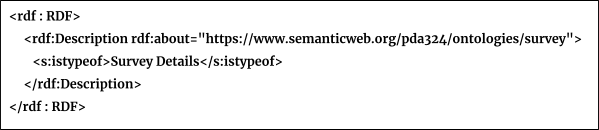
\includegraphics[width=15cm]{images/ch2/Figure4.png}
    \caption{An Illustration of Code in an RDF/XML Document}
    \label{fig:2.4}
\end{figure}
\par Figure~\ref{fig:2.5} shows an example of an \ac{rdf} as a triple. An \ac{rdf} triple, generally, follows subject-predicate-object format. For the illustration in the figure, the subject is \say{https://www.semanticweb.org/pda324/ontologies/survey}, predicate is \say{includes} and the object is \say{Survey Details}.
\begin{figure}[htp]
    \centering
    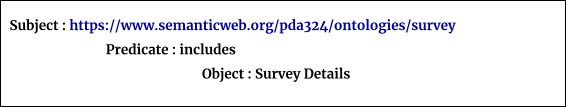
\includegraphics[width=15cm]{images/ch2/Figure5.png}
    \caption{An Example of an \ac{rdf} Triple}
    \label{fig:2.5}
\end{figure}
\par Figure~\ref{fig:2.6} show an \ac{rdf} in graphical format. Resource is indicated using an oval shape and a rectangle is used to represent a property value. A connector (an arrow) is used to represent a property to show that property (predicate) connects the resource (subject) with the value (object).
\begin{figure}[htp]
    \centering
    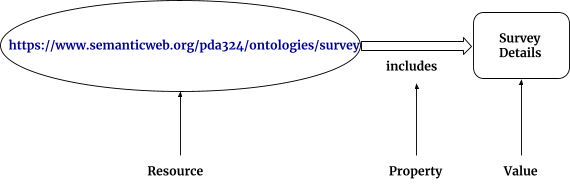
\includegraphics[width=15cm]{images/ch2/Figure6.png}
    \caption{Graphical Representation of an \ac{rdf}}
    \label{fig:2.6}
\end{figure}
\par The subject and object of the triples of \ac{rdf} act as nodes in the graph. In addition to \ac{rdf}/\ac{xml} documentation, the \ac{rdf} data model has a variety of serialization formats such as N-triples, which is a line base format where an \ac{rdf} triple is used to represent each line~\cite{beckett2014rdf}; \ac{turtle}; \ac{n3}, which is a subset of Turtle and N-Quads, which is an extension of N-Triples (line based) and adds a graph label to each line that allows multiple graph encoding~\cite{cyganiak2008n}.
\begin{table}[h!]
\centering
\begin{tabular}{| l | l |} 
 \hline
 Class/Property & Description  \\ 
 \hline
 rdfs:Resource & All things described by \ac{rdf} are called resources  \\ \hline
 rdfs:Class & The class of resources that are \ac{rdf} classes \\ \hline
 rdf:Property & The class of \ac{rdf} properties. It is an instance of rdfs:Class  \\ \hline
 rdfs:Literal & The class of literal values like integers and strings  \\ \hline
 rdfs:Datatype & The class of datatypes. All the objects of this class \\ & correspond to the \ac{rdf} model of datatype  \\ \hline
 rdf:HTML & The class of \ac{html} literal values and subclass of rdfs:Literal  \\ \hline
 rdfs:range & An instance of rdf:Property that is used to state that the \\ & values of a property are instances of one or more classes   \\ \hline
 rdfs:domain & An instance of rdf:Property that is used to state that any \\ & resource that has a given property is an instance of one or \\ & more classes. \\ \hline
 rdf:type & An instance of rdf:Property that is used to state that a \\ & resource is an instance of a class  \\ \hline
 rdfs:subClassOf & An instance of rdf:Property that is used to state that all the \\ & instances of one class are instances of another  \\ \hline
 rdfs:label & an instance of rdf:Property that may be used to provide a \\ &  human-readable version of a resource's name  \\ \hline
 rdfs:subPropertyOf \ \ & An instance of rdf:Property that is used to state that all \\ & resources related by one property are also related by another  \\ 
 \hline
\end{tabular}
\caption{Commonly used Classes and Properties of RDFS}
\label{table:2.1}
\end{table}
\par \ac{rdfs}, according to McBride~\cite{mcbride2004resource}, was introduced by the \ac{w3c} as a technique to define resource types and property names. The data publishers can use \ac{rdfs} to define various vocabularies in an \ac{rdf} model. Some of the commonly used \ac{rdfs} classes and properties\footnote{https://www.w3.org/TR/rdf-schema/} along with their description are listed in Table~\ref{table:2.1}~\cite{mcbride2004resource}.
\par Figure~\ref{fig:2.7} shows a graph for the representation of \ac{rdfs} for a comparatively complex and abstract example based on \ac{rdf} Primer~\cite{manola2004rdf}. The graph has been drawn for the following statement:
\emph{\begin{center}
    Romeo and Juliet is written by William Shakespeare.
\end{center} }
\par Figure~\ref{fig:2.7} is the graphical representation of an \ac{rdf} with schema as well as data. In the graph, the rdf:type of \say{Romeo and Juliet} is \say{Play} which in turn is an rdf:subClassOf \say{Literature}. Also, the rdf:type of \say{William Shakespeare} is \say{Person} which, further, is an rdfs:range of \say{is written by} of rdfs:domain \say{Literature}.
\begin{figure}[htp]
    \centering
    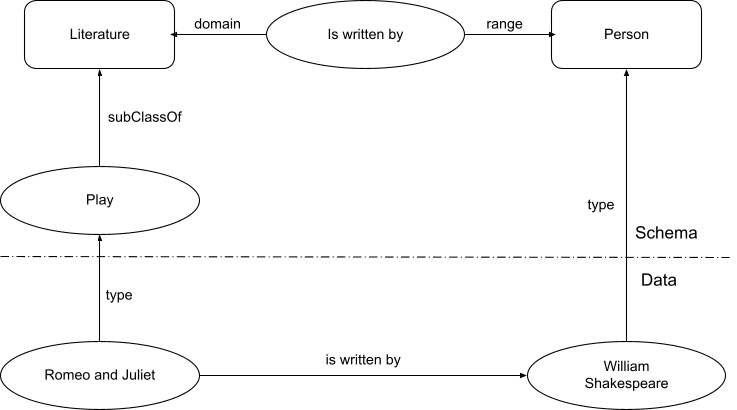
\includegraphics[width=15cm]{images/ch2/Figure7.png}
    \caption{Graphical Representation of an RDFS for a Comparatively Complex Illustration, after McBride~\cite{mcbride2004resource}}
    \label{fig:2.7}
\end{figure} 
\par The actual \ac{rdf} looks quite different from the previous example (Figures~\ref{fig:2.4}, ~\ref{fig:2.5}, ~\ref{fig:2.6} and ~\ref{fig:2.7}). For the representation of an actual \ac{rdf}, consider Figure~\ref{fig:2.8} for the corresponding English statement. \say{http://www.semanticweb.org/survey.html} is a subject \ac{uri} with respondent and Robert James having \ac{uri}s as \say{http://xyz.org/1/respondent} and \say{http://www.semanticweb.org/responseID/1234} respectively. The example represents a survey system which has responses as well as respondents and related details as a part of the environment.
\begin{figure}[htp]
    \centering
    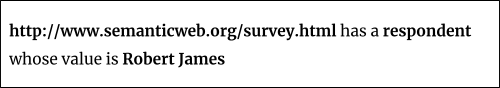
\includegraphics[width=15cm]{images/ch2/Figure8.png}
    \caption{English Statement for an Example of Actual \ac{rdf}}
    \label{fig:2.8}
\end{figure}
\par In the form of \ac{rdf} triple, the statement in Figure~\ref{fig:2.8} can be represented as shown in Figure~\ref{fig:2.9}. \ac{uri} is assigned to the subject survey.html and to the object which is the response with responseID 1234 which corresponds to the property value Robert James. A \ac{uri} is also assigned to the predicate (respondent).
\begin{figure}[htp]
    \centering
    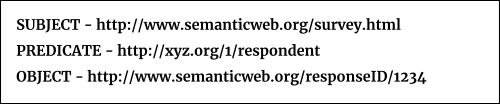
\includegraphics[width=15cm]{images/ch2/Figure9.png}
    \caption{\ac{rdf} Triple for English Statement in Figure~\ref{fig:2.8}, after \ac{rdf} Primer~\cite{manola2004rdf}}
    \label{fig:2.9}
\end{figure}
\par Figure~\ref{fig:2.10} shows a graphical representation of the \ac{rdf} triple in Figure~\ref{fig:2.9}. The subject and the object are two entities and the predicate being the third entity acts as a connector between them. Considering an entity-relationship data model, the predicate can be treated as a relationship shared by the subject and the object. There can be more details added to the system, that is, more statements can be added which are in relation to the one in Figure~\ref{fig:2.8}. Suppose the new statement added is:
\begin{center}
\par \emph{http://www.semanticweb.org/survey.html} has a \emph{date} with value \emph{Sept. 08, 2020}    
\end{center} and the \ac{uri} for the date is \say{http://www.semanticweb.org/respDetails/date}.
\begin{figure}[htp]
    \centering
    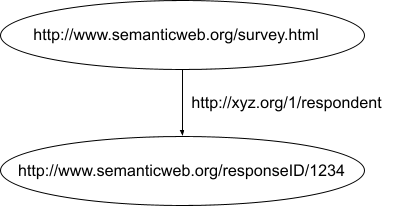
\includegraphics[width=14cm]{images/ch2/Figure10.png}
    \caption{\ac{rdf} Graph for English Statement in Figure~\ref{fig:2.8}, after \ac{rdf} Primer~\cite{manola2004rdf}}
    \label{fig:2.10}
\end{figure}
\par The new graph would be as shown in Figure~\ref{fig:2.11} where as the set of statements in Table~\ref{table:2.2} shows the \ac{rdf} triple notation for Figure~\ref{fig:2.11}. The first notation represents the entities, survey.html (subject) and Robert James (object), along with respondent (predicate) as the relation between them, using the \ac{uri}s. The second notation is for the date, where instead of the \ac{uri}, the value of the property, Sept. 08, 2020, is used. Here, survey.html is the subject and Sept. 08, 2020 is the object with date acting as the predicate.
\begin{figure}[htp]
    \centering
    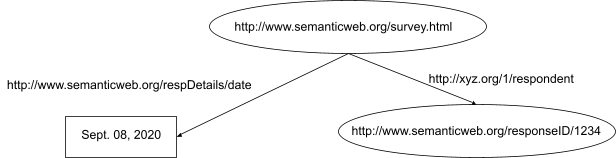
\includegraphics[width=15cm]{images/ch2/Figure11.png}
    \caption{\ac{rdf} Graph for Two Relative Statements, after \ac{rdf} Primer~\cite{manola2004rdf}}
    \label{fig:2.11}
\end{figure}
\begin{table}[h!]
\centering
\begin{tabular}{|l|} 
 \hline
  \ \ <http://www.semanticweb.org/survey.html> <http://xyz.org/1/respondent> \\ \ \ <http://www.semanticweb.org/responseID/1234> . \\ \hline
 \ \ <http://www.semanticweb.org/respDetails/date> “Sept. 08, 2020” . \\ \hline
\end{tabular}
\caption{\ac{rdf} Notations for Figure~\ref{fig:2.11}, after \ac{rdf} Primer~\cite{manola2004rdf}}
\label{table:2.2}
\end{table}
\par Consider a more complex system, where the details of respondent are collected. Suppose, one of the details is name and the other is address of the respondent.  Figure~\ref{fig:2.12} shows a graphical representation of this \ac{rdf} system.
\begin{figure}[htp]
    \centering
    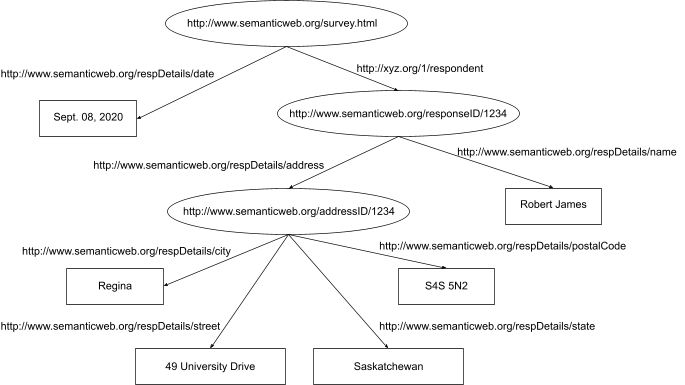
\includegraphics[width=15cm]{images/ch2/Figure12.png}
    \caption{Graphical Representation of \ac{rdf} with Details of the Respondent of the Survey, after \ac{rdf} Primer~\cite{manola2004rdf}}
    \label{fig:2.12}
\end{figure}
%% \marginpar{"after \ac{rdf} Primer" -- this appears a lot. I would like to see  consistency of text sizes and styles, perhaps using \LaTeX directly instead of images...} it is just that the information can be represented in 5 figures and 1 table after reading RDF Primer
\par For name, the respondent is subject and Robert James acts as object whereas respName is the predicate. The \ac{uri} for respName is \say{http://www.semanticweb.org/respDe- tails/name} and the value, Robert James, is the object. On the other hand, respondent (subject) is connected to address (object) node, with \ac{uri} \say{http://www.semanticwe- b.org/addressID/1234}, through respAddress (predicate) with \ac{uri} \say{http://www.sema- nticweb.org/respDetails/address}. Further, the address node has multiple child nodes, namely, street, city, state and postal code. The address (subject) \ac{uri} is connected to the values of four different object values, 49 University Drive (street), Regina (city), Saskatchewan (state) and S4S 5N2 (postalCode) where the \ac{uri}s for the predicates are \say{http://www.semanticweb.org/respDetails/street}, \say{http://www.semanticweb.org/res- pDetails/city}, \say{http://www.semanticweb.org/respDetails/state} and \say{http://www.se- manticweb.org/respDetails/postalCode} respectively. Instead of using an unnecessary \ac{uri} for the address entity, a blank node can be used to denote the entity, as shown in Figure~\ref{fig:2.13}. As the relationships of the node with other nodes give sufficient details without hindering the flow of the data tree, the node does not require a \ac{uri}reference\footnote{https://lists.w3.org/Archives/Public/uri/2007Jul/0027.html}.
\begin{figure}[htp]
    \centering
    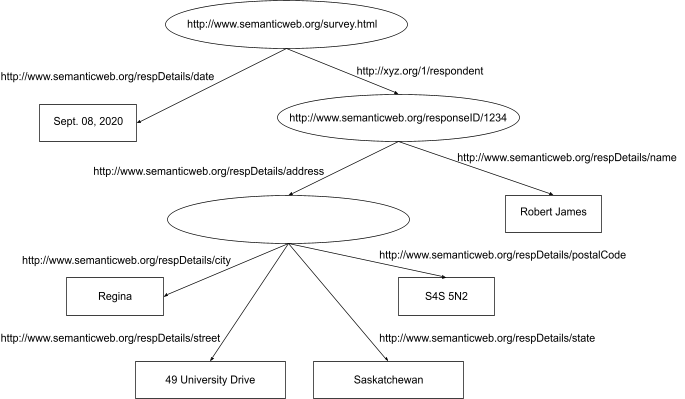
\includegraphics[width=15cm]{images/ch2/Figure13.png}
    \caption{\ac{rdf} Representation in Figure~\ref{fig:2.12} without a URI (blank node) for Address Entity, after \ac{rdf} Primer~\cite{manola2004rdf}}
    \label{fig:2.13}
\end{figure}
\par In 2004, \ac{w3c} recommended intended goals that are to be achieved whenever an \ac{rdf} is to be designed. According to the \ac{w3c}Recommendation\footnote{https://www.w3.org/TR/rdf-concepts/}, the design should \say{have a simple data model; formal semantics and provable inference; should use an extensible \ac{uri}-based vocabulary and an \ac{xml}-based syntax; should support the use of \ac{xml} schema datatypes; and should allow any one to make statements about any resource}.
\subsection{Uniform Resource Identifier} \label{subsection:uri}
\par An abstract (a logical) or a physical resource on the web is identified by a unique set of ASCII characters which is referred to as a \ac{uri}\footnote{https://www.w3.org/wiki/URI}. According to Berners-Lee et. al.~\cite{berners1998uri} in RFC 3986, the unique string, on the web, follows a set of guidelines and security considerations while defining a syntax for the generic \ac{uri} and determining a process for \ac{uri} references' resolution. As mentioned by \ac{w3c}, for the operating systems on \ac{uri}s, some specific \say{protocols are defined depending on the UriScheme\footnote{https://www.w3.org/2001/tag/doc/SchemeProtocols.html}}. A system can perform multiple operations like \say{access}, \say{update}, \say{replace} and \say{find attributes} on the identified resources. In RFC 2396, Berners-Lee et al.~\cite{fielding1998uri} characterized \ac{uri} using three definitions, as shown in Table~\ref{table:2.3}.
\begin{table}[h!]
\centering
\begin{tabular}{| l | l |} 
 \hline
 Term & \ \ \ \ \ \ \ \ \ \ \ \ \ \ \ \ \ \ \ \ \ \ \ \ \ \ \ \ \ \ \ \ \ \ \ \ \ \ \ \ Definition  \\ 
 \hline
  \multirow{9}{4em}{Uniform} & There are various benefits of achieving uniformity, like, it facilitates\\ & different procedures to access resources in the same environment using\\ & different types of resource identifiers; new types of resource identifiers\\ & can be introduced without modifying the actual usage of the existing\\ & identifiers; common syntactic conventions can be interpreted uniformly\\ & for a variety of resource identifiers on the semantic web; and the new\\ & applications or protocols can utilize the already existing large and\\ & widely-used resource identifiers as the identifiers can be reused in\\ & different contexts. \\ \hline
 \multirow{9}{0em}{Resource} & Anything on the web that can be uniquely identified is referred to as\\ & a resource. Some day-to-day examples of a resource are a computeri-\\ & zed file or folder, weather-broadcasting service, an image, and a set of\\ & other resources. Some resources like books in a library, an animal, a\\ & human being,and a corporation are a set of resources that cannot be\\ & retrieved over the network. A resource is the \say{conceptual mapping}\\ &~\cite{fielding1998uri} to a set of entities independent of the corresponding entities at a\\ & particular time. Hence, if the conceptual mapping isn't changed, a\\ & resource can remain constant irrespective of the changes in its content.\\ \hline
 \multirow{3}{0em}{Identifier} & An object which is used as a reference to a thing with unique identity\\ & on the web is termed as an identifier. In \ac{uri}, a string of ASCII char-\\ & acters restricted by a specific syntax is object.\\ \hline
\end{tabular}
\caption{Definitions Used for Characterizing URI, by Berners-Lee et al.~\cite{fielding1998uri}}
\label{table:2.3}
\end{table}  
\subsubsection{Syntax of a \ac{uri}}
\par According to Berners-Lee et al.~\cite{berners1998uri}, the generic syntax of a \ac{uri} comprises five components in a hierarchical sequence which are as follows:
\begin{center}
\par \ac{uri} = scheme: [//authority] path [?query] [\#fragment]    
\end{center}
where the authority component consists of three more components which are:
\begin{center}
\par authority = [userinfo@] host [:port]
\end{center}
\par A syntax diagram can be modelled to represent the components of Generic Syntax\footnote{https://www.w3.org/Addressing/URL/uri-spec.html} of \ac{uri} along with their hierarchy as shown in Figure~\ref{fig:2.14}. Consider the following \ac{url}. Figure~\ref{fig:2.15} shows its components.
\begin{center}
\par https://parita@www.semanticweb.org:695/ontology/?tag=survey\&order=newest\#top
\end{center}
\begin{figure}[htp]
    \centering
    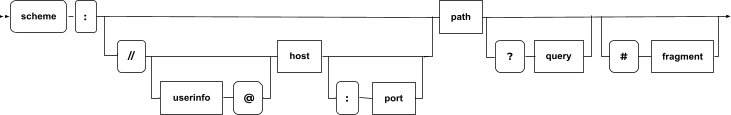
\includegraphics[width=15cm]{images/ch2/Figure14.png}
    \caption{Syntax Diagram of a Generic URI, after Berners-Lee et al.~\cite{berners1998uri}}
    \label{fig:2.14}
\end{figure}
\begin{figure}[htp]
    \centering
    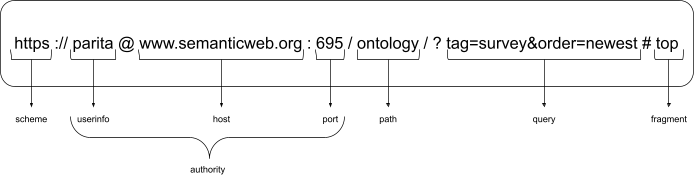
\includegraphics[width=15cm]{images/ch2/Figure15.png}
    \caption{Components of an Example of URL, after Berners-Lee et al.~\cite{berners1998uri}}
    \label{fig:2.15}
\end{figure}
\section{Linked Data Life Cycle}
\par The Linked Data Life Cycle includes multiple stages as described by Ngomo et al.~\cite{ngomo2014introduction} which are listed in Table~\ref{table:2.4}. Each stage of this life cycle is independent yet linked to one another. So, it is not mandatory to go through all the stages sequentially to publish the data on the web. It is necessary to use a procedure that follows the life cycle to ensure the quality of data to be published as linked data. The first stage, generally, is data extraction along with conversion of the extracted data (in forms other than \ac{rdf}) into \ac{rdf}. Once the data is in \ac{rdf} form, any or all of the other stages listed in Table~\ref{table:2.4} can be performed.
\begin{table}[h!]
    \centering
    \begin{tabular}{|l|l|} 
    \hline Stage \ & Description \\ \hline
     Extraction & Extraction and conversion of unstructured and semi-\\ & structured data into \ac{rdf}\\ \hline
     Storage \& Querying & Storing the \ac{rdf} data in a format that supports data\\ & querying efficiently\\ \hline
     Authoring & Allowing the users to create new data or to access and\\ & modify the existing data\\ \hline
     Linking & Creating links the data belonging to various domains\\ & and users based on their entities\\ \hline
     Enrichment & Data enrichment for efficient query support using\\ & various top-tier structures\\ \hline
     Quality Analysis & Managing data using different strategies to ensure good\\ & quality of available data on the web\\ \hline
     Browsing \& Exploration & Making the structured data available on the web for\\ & the users to browse and explore effectively\\ \hline
    \end{tabular}
    \caption{Stages in Linked Data Life Cycle, after Ngomo et al.~\cite{ngomo2014introduction}}
    \label{table:2.4}
    \end{table}
\section{Conversion of Data from CSV to \ac{rdf}}
\par The preferred format of the data published on the semantic web is \ac{rdf} format. Many data scientists use tables and spreadsheets to store and publish data using \ac{csv} files over \ac{rdf} format as conversion of data to \ac{rdf} is comparatively difficult. The data used by Dr. Hepting has been stored in tabular format (Sample \ac{csv} data consisting of all responses is available in Appendix~\ref{chap:appendix1} ). To convert tabular data into \ac{rdf} (Appendix~\ref{chap:appendix2} consists of \ac{rdf} code for the \ac{csv} data in Appendix~\ref{chap:appendix1}), \ac{w3c}\footnote{https://www.w3.org/wiki/ConverterToRdf} recommends the following open source tools~\cite{ermilov2013csv},
\begin{itemize}
    \item OpenRefine:
    \par OpenRefine\footnote{https://openrefine.org}, an \ac{rdf} extension of Google Refine, is a powerful java-based set of tools that work with messy data using \ac{grel}\footnote{https://libjohn.github.io/openrefine/grel.html}. It allows the users to extract, transform, export, and convert \ac{csv}, Ex cel, spreadsheets and other tabular data into \ac{rdf} where a \ac{gui} is used to define schema mapping.
    \item RDF123:
    \par RDF123\footnote{https://ebiquity.umbc.edu/resource/html/id/237/RDF123-java-application-v1-0} is a java application and servlet for the conversion of \ac{csv} and spreadsheets to \ac{rdf} which uses arbitrary graphs to define schema mapping. According to Han et. al~\cite{han2008rdf}, it uses a graphical RDF123 template to allow users to convert the data from spreadsheets to \ac{rdf}.
    \item csv2rdf4lod:
    \par csv2rdf4lod\footnote{https://github.com/timrdf/csv2rdf4lod-automation/wiki} is a tool that is used for the conversion of tabular data into structured and linked \ac{rdf} using specifications that are based on declarative \ac{rdf} enhancement parameters. It forms default namespaces for \ac{uri}s and provides VoID and original metada for the conversion using identifiers for source organization, dataset and version.
    \item XLWrap:
    \par XLWrap\footnote{https://xlwrap.sourceforge.io} is a graphical template based application that allows execution of various \ac{sparql} queries~\cite{andreas2009xlwrap}.  The spreadsheets are wrapped to arbitrary \ac{rdf} graphs which allows:
    \begin{itemize}
    	\item Streamed processing of tabluar data like Excel, OpenDocument and \ac{csv}
	\item Loading Local/\ac{http}
	\item Expressions that include calculator operations for Excel and OpenDocument, and Custom functions
	\item Use of \ac{api} and \ac{sparql} endpoint
    \end{itemize}
    \item Tarql:
    \par Tarql\footnote{https://tarql.github.io} operates as a command-line application for the conversion of \ac{csv} to \ac{rdf} using a user-defined mapping that is written in \ac{sparql} standard 1.1.
\end{itemize}
\section{Ontology Editors}
\par Ontology editors are used by publishers to create new ontologies when the existing vocabulary is not suitable for their purpose. \ac{w3c}\footnote{https://www.w3.org/wiki/Ontology\_editors} has recommended a list of ontology editors that can be used to edit, manage, organize and visualize ontology. The list of editors includes Protégé, NeOn Toolkit, SWOOP, Neologism, TopBraid Composer, Vitro, Knoodl, Anzo for Excel, OWLGrEd, Fluent Editor, Semantic Turkey, VocBench. The page does not include valid links to the editors' websites. Protégé is the most popular ontology editor among researchers. There exists negligible information about most of the editors in the list which has driven the decision of the use of Protégé for ontology development and OntoGraf and WebVOWL for visualization.
\section{Applications of Linked Open Data}
\par A variety of projects and websites, that use linked open data, have been developed. Wikidata and DBpedia are two major projects of linked open data that present structured data on the semantic web. This section consists of a brief description of both applications.
\subsection{Wikidata}
\par According to a report by Krotzsch and Vrandecic~\cite{denny2014wikidata}, Wikidata was introduced to the world of information engineering in 2012 by Wikimedia. Wikidata can be defined as \say{the community-created
knowledge base of Wikipedia and the central data management platform for
Wikipedia and most of its Sister Projects\footnote{Wikipedia, Wikivoyage, Wiktionary, Wikisource, and others}}, according to Erxleben et al.~\cite{fredo2014intro}. Wikidata was established for the collection and integration of data on the semantic web with Wikipedia. Wikidata is a free open-source tool that handles a large amount of structured data and maintains pages that store the data. Each entity on Wikidata represents the subject of a triple with a dedicated page. The properties of Wikidata are similar to that of \ac{rdf} where the individuals and classes are indicated using items. As Wikidata is an open-source tool, the data on a page of the Wikidata is easily available for the users to access as well as edit.
\par For instance, the University of Regina, a university in the provincial capital of Saskatchewan—the city of Regina, has an item page allotted for it. Figure~\ref{fig:2.16} shows the Wikidata item page of the University of Regina that can be accessed using the link: https://www.wikidata.org/wiki/Q3104287. Wikidata uses a method of automatically assigning unique identifiers to the entities, which are used as the labels of the item pages instead of the actual names of the entities. These identifiers are a string starting with a capital Q followed by a sequence of digits. The identifiers are assigned irrespective of the language as the Wikidata website supports multiple languages. For the University of Regina, the label used is \say{Q3104287}. The item page on Wikidata consists of multiple sections:
\begin{itemize}
    \item label: The name of the subject that is treated as an entity. For the instance in Figure~\ref{fig:2.16}, the label is \say{University of Regina} along with the unique identifier \say{Q3104287}. 
    \begin{figure}[htp]
    \centering
    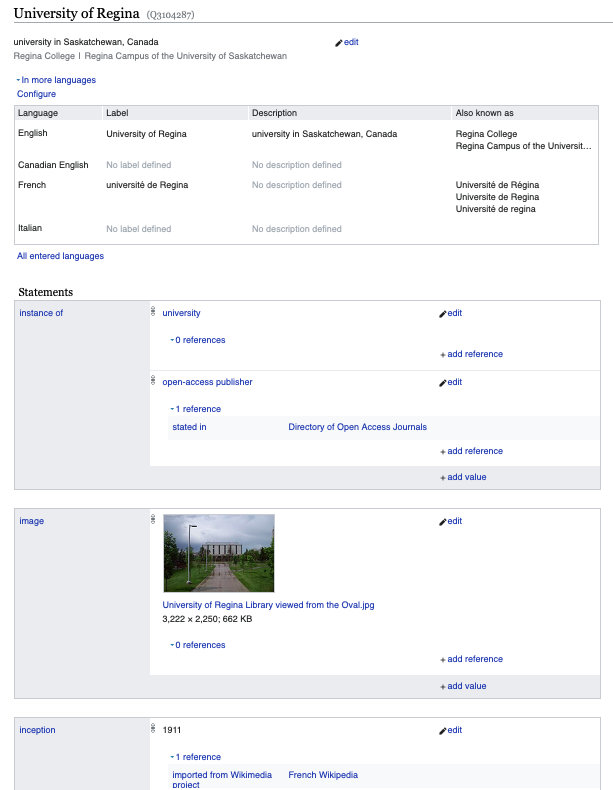
\includegraphics[width=15cm]{images/ch2/Figure16.png}
    \caption{Details of University of Regina, Regina, SK on Wikidata}
    \label{fig:2.16}
\end{figure}
    \item description: This section consists of general introductory details about the subject. For the University of Regina, the description on wikidata is \say{university in Saskatchewan, Canada}.
    \item statements: This section consists of a list of subsections called \say{property}. The properties along with their property IDs for the University of Regina are listed in Table~\ref{table:2.5}.
    \begin{table}[h!]
    \centering
    \begin{tabular}{|l|l|} 
    \hline Statement Property \ & Property ID \\ \hline
     instance of & P31\\ \hline
     image & P18\\ \hline
     inception & P571\\ \hline
     country & P17\\ \hline
     located in the administrative territorial entity & P131\\ \hline
     coordinate location & P625\\ \hline
     subsidiary & P355\\ \hline
     official website & P856\\ \hline
     commons category & P373\\ \hline
     topic's main category & P910\\ \hline
     category for employees of the organization & P4195\\ \hline
     category for alumni of educational institution & P3876\\ \hline
     API endpoint & P6269\\ \hline
     social media followers & P8687\\ \hline
    \end{tabular}
    \caption{Statement Properties and Property IDs for the University of Regina on Wikidata}
    \label{table:2.5}
    \end{table}
    \item identifiers: This section consists of various IDs belonging to the subject. For the University of Regina, the set of properties used for identifiers and their IDs are listed in Table~\ref{table:2.6}.
    \begin{table}[h!]
    \centering
    \begin{tabular}{|l|l|} 
    \hline Identifier Property \ & Property ID \\ \hline
     VIAF ID & P214\\ \hline
     ISNI & P213\\ \hline
     GND ID & P227\\ \hline
     Library of Congress authority ID & P244\\ \hline
     WorldCat Identities & P7859\\ \hline
     ARWU university ID & P5242\\ \hline
     Crossref funder ID & P3153\\ \hline
     Facebook ID & P2013\\ \hline
     Freebase ID & P646\\ \hline
     Google Maps Customer ID & P3749\\ \hline
     GRID ID & P2427\\ \hline
     HAL structure ID & P6773\\ \hline
     LittleSis organization ID & P3393\\ \hline
     Microsoft Academic ID & P6366\\ \hline
     Ringgold ID & P3500\\ \hline
     ROR ID & P6782\\ \hline
     Times Higher Education World University ID & P5586\\ \hline
     Twitter username & P2002\\ \hline
     U-Multirank university ID & P5600\\ \hline
    \end{tabular}
    \caption{Identifier Properties and Property IDs for University of Regina on Wikidata}
    \label{table:2.6}
    \end{table}
\end{itemize}
\par The \ac{uri} for an entity on Wikidata is \say{https://www.wikidata.org/wiki/<id>}, where <id> stands for the unique identifier. For the University of Regina, the <id> is the label identifier—Q3104287. Figure~\ref{fig:2.17} shows the \ac{rdf}/\ac{xml} description of the University of Regina on Wikidata.
\begin{figure}[htp]
    \centering
    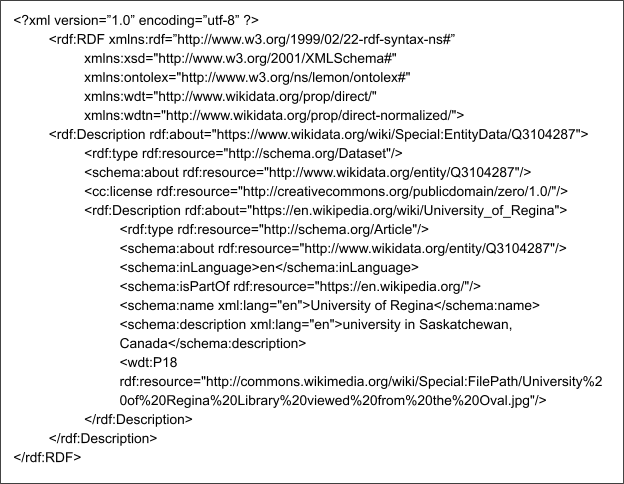
\includegraphics[width=15cm]{images/ch2/Figure17.png}
    \caption{Wikidata Entry (RDF/XML) for University of Regina, Regina, SK}
    \label{fig:2.17}
\end{figure}
\subsection{DBpedia}
\par Jimmy Wales and Larry Sanger, in 2001, created the largest general reference work on the internet consisting of articles\footnote{include data comprising of templates, images, videos, categorizations, and links to other articles (pages) in multiple languages} in over 280 languages, the Wikipedia\footnote{https://en.wikipedia.org/wiki/Main\_Page}, which acts as a source of data for many web projects like DBpedia\footnote{https://wiki.dbpedia.org/}, one of the major linked open data projects. The main aim behind the development of DBpedia is the conversion of unstructured data on Wikipedia into structured datasets. DBpedia enables querying the Wikipedia data as well as the generation of links among the structured datasets, resulting in the establishment of a massive web of data.
\par Initially, the template of the page is discovered using a Template Extraction Algorithm\footnote{like Principle Components Analysis, Linear Discriminant Analysis, Logically Linear Embedding} which results in the identification of the structure of the template using various Pattern Matching Techniques\footnote{https://www.dummies.com/programming/big-data/data-science/how-pattern-matching-works-in-data-science}. Once the appropriate template is selected, the template data is parsed using a suitable algorithm and transformed into \ac{rdf} triples. MediaWiki\footnote{https://www.mediawiki.org/wiki/MediaWiki} links are identified and assigned specific \ac{uri}s. On the other hand, the common units of data are recognized  and assigned appropriate datatypes whereas \ac{rdf} lists are created for the object lists. According to Auer et al.~\cite{auer2007dbpedia}, DBpedia in 2007 was a platform that delivered information on \say{more than 1.95 million \say{things} that includes at least 80,000 persons, 70,000 places, 35,000 music albums, 12,000 films}. The DBpedia semantic web services are handled using the GNU Free Documentation License terms and policies. The data on DBpedia is easily accessible in different ways like accessing the datasets as linked data; using \ac{sparql} queries for data extraction and accessibility; and in the form of a downloadable \ac{rdf} snippets~\cite{bizer2009dbpedia}. Figure~\ref{fig:2.18} shows DBpedia entry for the \say{University of Regina, Regina, SK}. Like Wikidata, DBpedia also has a label, a description section and a set of important property-value pairs that give information related to the entity that has been described.
\begin{figure}[htp]
\centering
    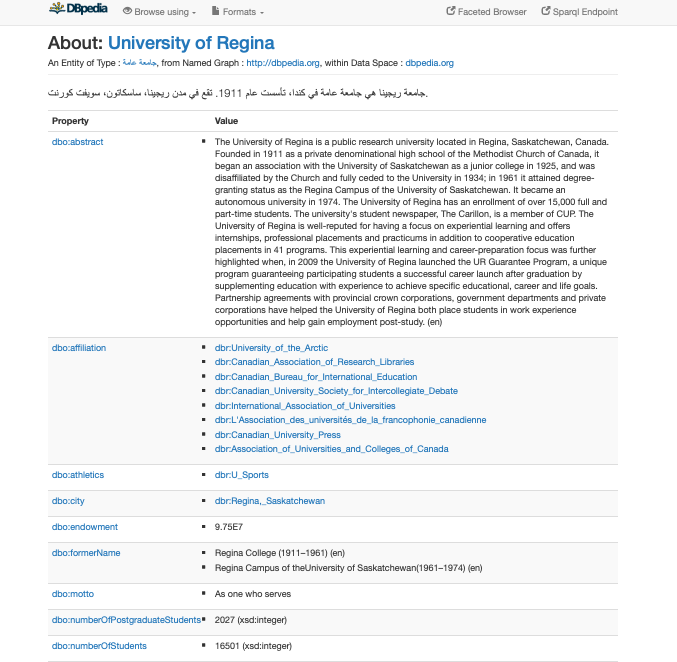
\includegraphics[width=15cm]{images/ch2/Figure18.png}
    \caption{Description of University of Regina, Regina, SK on DBpedia}
    \label{fig:2.18}
\end{figure}
\par Figure~\ref{fig:2.19} shows the data architecture of DBpedia. An open-link software, Virtuoso Universal Server\footnote{https://dbpedia.org/page/Virtuoso\_Universal\_Server}, is a data virtualization tool used to host and publish \ac{rdf} datasets on DBpedia, which can be easily accessed using \ac{sparql} endpoint. The \ac{html} or \ac{rdf} representation of the DBpedia resources is enabled by the data architecture using \ac{http} that supports the standard \ac{http} GET method calls from the web clients.
\begin{figure}[htp]
    \centering
    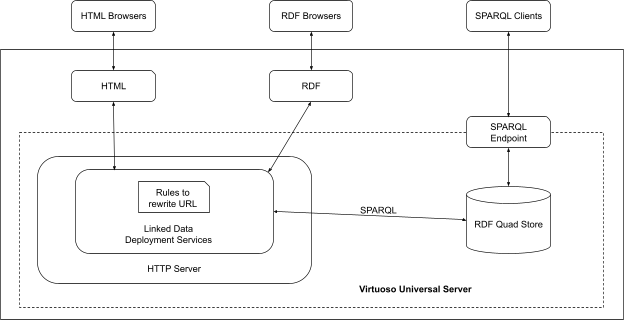
\includegraphics[width=15cm]{images/ch2/Figure19.png}
    \caption{DBpedia Data Architecture}
    \label{fig:2.19}
\end{figure}
\end{doublespace}



%!TEX root = parita-msc.tex
\chapter{Proof Of Concept}
\label{chap:proofOfConcept}
\begin{doublespace}
\par This chapter focuses on some fundamental concepts of \ac{owl} ontologies that were considered while developing the survey instrument for this research work. 
\section{Ontology in Web Semantics}
\par Ontology is a branch of information science that encloses representation, nomenclature, and definition of various properties, categories, and relationships shared among the entities\footnote{includes all types of data, concepts and entities} that support any number of domains the user is interested in. In other words, Ontology is a form of defining a set of concepts for representing the subject properties and the relationships shared among them. According to Tom Gruber~\cite{gruber1995towards}, ontology is \say{an explicit specification of a conceptualization}, where conceptualization is \say{an abstract, simplified view of the world (includes objects, concepts and other entities that are assumed to exist in some area of interest and the relationships that hold among them) that we wish to represent for some purpose}. In web semantics, an ontology is used to define the semantics of the resources briefly and methodically. The ontologies have have been used to \say{specify the physical as well as conceptual characteristics of resources, in the form of metadata schema on the semantic web, for a fixed set of users}~\cite{jacob2003ontologies}.
\section{\ac{owl} Ontologies}
\par W3C developed a standard ontology language called \ac{owl}\footnote{ http://www.w3.org/TR/owl- guide/} to define and describe concepts for ontology using different facilities and operations like intersection, union and negation. It is based on a logical model due to which a reasoner\footnote{maintains hierarchy accurately} can be used to check the mutual consistency among the statements and definitions in the ontology. The reasoner is also responsible for the identification of a suitable concept for particular definitions~\cite{horridge2009practical}.
\subsection{Components of \ac{owl} Ontologies}
\par An \ac{owl} ontology consists of a set of components that define and describe the concepts collectively. The basic components of any \ac{owl} ontology, Individuals, Properties and Classes, are briefly explained in this section.
\begin{itemize}
    \item Individuals:
    \par According to Horridge et al.~\cite{horridge2009practical}, \say{Individuals represent objects in the domain in which we are interested}. Individuals are the objects of classes. Figure~\ref{fig:3.1} shows the representation of different individuals in various domains. The triangles are used here to denote the individuals in free space.
    \begin{figure}[htp]
    \centering
    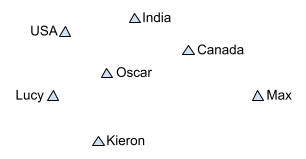
\includegraphics[width=8cm]{images/ch3/Figure1.png}
    \caption{Representation of Individuals in OWL}
    \label{fig:3.1}
\end{figure}
    \item Properties:
    \par The Binary Relationships\footnote{links shared by two individuals} between the individuals (things) are called properties. For instance, the individuals \say{Max} and \say{Kieron} from Figure~\ref{fig:3.1} are linked to each other by the property \say{hasSibling}. Each property can have its inverse. For instance, \say{hasSibling} can have an inverse property \say{isSiblingOf}. The properties can be symmetric or transitive. It is possible to have functional properties where the properties can be restricted to having only one value. Figure~\ref{fig:3.2} shows representation of properties between the individuals \say{Max} and \say{India}, and \say{Max} and \say{hasSibling}. The relation between \say{Max} and \say{India} is \say{livesIn}. The arrow between two individuals in the figure denotes the property (relationship) between them.
    \begin{figure}[htp]
    \centering
    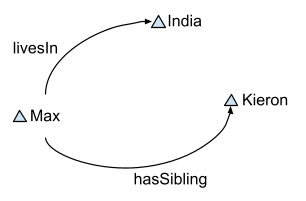
\includegraphics[width=8cm]{images/ch3/Figure2.png}
    \caption{Representation of Properties in OWL}
    \label{fig:3.2}
\end{figure}
    \item Classes:
    \par In \ac{owl}, the sets consisting of individuals are called \ac{owl} classes. Mathematical (formal) descriptions are used to describe the \ac{owl} classes. These descriptions include accurate statements on the requirements for the class membership. For instance, the class \say{Country} consists of all the individuals that are countries in the Domain of Discourse\footnote{can contain one or more classes}. Inheritance in \ac{owl} classes (Class Hierarchy) may exist with the classes having subclasses and/or super-classes which is technically termed as taxonomy. \say{Subclasses specialise (\say{are subsumed by}) their super-classes}~\cite{horridge2009practical}. For instance, consider the classes \say{Lady} and \say{Human}, where \say{Lady} is a subclass of \say{Human}. This implies the following statements:
    \begin{itemize}
        \item All ladies are humans
        \item All members of class \say{Lady} are members of class \say{Human}
        \item Being a \say{Lady} implies that individual is \say{Human}
        \item \say{Lady} is subsumed by \say{Human}
    \end{itemize}
    Figure~\ref{fig:3.3} shows the representation of the classes for the individuals and properties that are shown in Figure~\ref{fig:3.2}.
    \begin{figure}[htp]
    \centering
    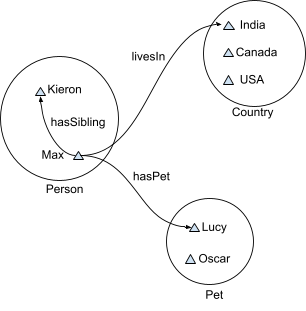
\includegraphics[width=8cm]{images/ch3/Figure3.png}
    \caption{Representation of OWL Classes Consisting of Individuals and Properties}
    \label{fig:3.3}
\end{figure}
\end{itemize}
\section{\ac{owl} Ontology Inconsistencies and Reasoner}
\par A Reasoner\footnote{https://en.wikipedia.org/wiki/Semantic\_reasoner} is used in Protégé to address and solve the inconsistencies. The current version of the Protégé \ac{ide} offers support for some built-in semantic reasoners which are listed below: 
\begin{itemize}
    \item ELK 0.4.3\footnote{https://www.w3.org/2001/sw/wiki/ELK} : A Java-based fast reasoner for lightweight \ac{owl}2 EL which is available under Apache License 2.0
    \item FaCT++ 1.6.5\footnote{https://www.w3.org/2001/sw/wiki/Fact} : A Tableaux-based reasoner for expressive \ac{owl} \ac{dl} which is implemented using C++
    \item HermiT 1.4.3.456\footnote{https://www.w3.org/2001/sw/wiki/Hermit} : A Java-based reasoner, written using \ac{owl}, that can be used to determine consistency of the ontology as well as for the identification of relationships among the classes of the ontology
    \item Mastro DL-Lite\footnote{https://protegewiki.stanford.edu/wiki/Mastro\_DL-Lite\_Reasoner} : An \ac{obda} management system in which the \ac{dl}-Lite family of languages for lightweight \ac{dl} are used for ontology specifications
    \item Ontop 4.1.0\footnote{https://www.w3.org/2001/sw/wiki/Ontop} : A reasoner which uses \ac{sparql} for querying datasets as Virtual \ac{rdf} Graphs
    \item Pellet and Pellet (incremental)\footnote{https://www.w3.org/2001/sw/wiki/Pellet} : A Java-based \ac{owl}2 reasoner for the optimization of nominals, conjunctive query answering, and incremental reasoning
\end{itemize}

\end{doublespace}
%!TEX root = parita-msc.tex

\chapter{\ac{owl} Ontology for Survey}
\label{chap:ontology}
\begin{doublespace}
\section{Development Tool for the Creation of New \ac{owl} Vocabularies}
\par In data science, for a fresh and developing branch like ontology engineering, it is difficult to find enough knowledge that can be reused. The field is still growing with research and development in progress as well as a lot still required to be explored in the future. As a result of this, linked open vocabularies are limited currently, and hence, the data publishers will have to create a vocabulary in case they do not find the required vocabulary from the already existing vocabularies.
\par There are editors available today that help the publishers to create their own linked open vocabularies. Alatrish at the University of Belgrad~\cite{alatrish2013comparison}, in 2013, compared the most used ontology editors, namely, Apollo, OntoStudio, Protégé, Swoop, and TopBraid Composer. The editors were compared based on the following features:
\begin{itemize}
  \item General description: developers' details, and accessibility on the internet (open source or software licensed)
  \item Software architecture and tools evaluation: semantic web architecture, support for plug-ins, backup management, and ontology storage
  \item Interoperability: interoperability with other ontology tools, support and translation for other languages
  \item Knowledge representation: Knowledge Representation (KR) paradigm of knowledge model, axiom language, and methodological support
  \item Inference services: built-in inference engine, other attached inference engines, and constraint/consistency checking
  \item Usability: graphical taxonomy, graphical views, zooms, collaborative working, and ontology libraries
\end{itemize}
\par After studying the details and comparison among the most used editors based on the above features by Alatrish~\cite{alatrish2013comparison}, Protégé has been used for the development of the instrument to support this research and thesis work.
\section{Protégé}
\par Stanford University developed a free, open-source ontology development platform, Protégé\footnote{https://protege.stanford.edu}, that offers a set of substantial tools\footnote{along with various plug-ins and Java-based \ac{api}} to build ontologies for knowledge-based applications and to implement various \say{knowledge-modeling structures and actions that support the creation, visualization and manipulation of ontologies in various representation formats}~\cite{alatrish2013comparison}. Protégé offers customization options to build knowledge models and to add data. 
\subsection{Usability of Protégé}
\par The \ac{iso} standard 9241\footnote{https://www.iso.org/standard/63500.html} defines usability as \say{the extent to which a product can be used by specified users to achieve specified goals with effectiveness, efficiency, and satisfaction in a specified context of use}. In usability engineering, Jacob Neilson~\cite{neilson1994usability} suggested five qualities of a usable product: \say{learnability, efficiency, memorability, errors (low rate,
easy to recover), and satisfaction}. These were the original five dimensions of usability which were then re-termed as all five words starting with \say{E} by Quesenbery~\cite{quesenbery2003dimensions}, and they became popular as the five Es of usability~\cite{quesenbery2003dimensions}. The new terms are as shown in Figure~\ref{fig:4.1}.
\begin{figure}[htp]
    \centering
    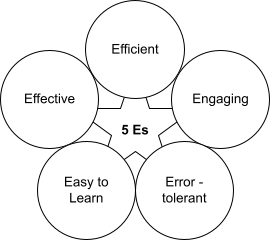
\includegraphics[width=12cm]{images/ch4/Figure1.png}
    \caption{Five Es of Usability}
    \label{fig:4.1}
\end{figure}
\begin{itemize}
  \item Effective: The task is completed accurately
  \par The user must be able to complete the desired task accurately using the design. If the user is unable to complete the task, irrespective of the time spent and efforts made to complete the task, the design is said to have failed to reach meet the design's goals. To measure effectiveness in a design, it is necessary to know users' perspectives of success and accuracy.
  \item Efficient: The task is completed quickly
  \par The user must be able to complete the task easily. The interface should be designed to allow the users to complete the desired tasks with the least complexity and within the minimum possible time. If a simple task takes more than the required time for completion, the design is not feasible and would be said to not meet the goals.
  \item Engaging: The look and feel of the design is interactive and engaging
  \par The look and feel of the interface must be interactive so that the user finds it interesting and continues using it. The user of the interface should be able to connect with the presentation and the organization of the components of the interface and hence should be satisfied by using the design to complete the desired task.
  \item Error-tolerant: Error prevention and data recovery in case any error is committed
  \par The interface should be able to easily handle errors. This means in case the user commits mistakes, the interface should be helpful enough to not lose the work done by the user along with providing the error correction options.
  \item Easy to learn: The interface should be easy to learn
  \par The user should get the feeling of familiarity and adaption while using the interface. The names of the components and tools in the design must be appropriate so that the user can understand their purpose from the name itself. For instance, in a banking application, using the keyword \say{balance owed} to denote the debit amount might confuse the user by not giving a clear idea about who owes the money, that is, whether the customer owes the amount to the bank or vice versa.
\end{itemize}
\par The five dimensions of usability can be considered while designing as well as for evaluation. While designing, the engineers consider the five dimensions as goals to be achieved whereas while testing and evaluation, they are considered as the requirements necessary for the designed model. The five dimensions of usability were used to assess the usability of Protégé and the report of the evaluation is as follows:
\begin{itemize}
  \item Effective: Protégé is an effective design as it allows the users to build ontologies and use other tools precisely. The users can complete the desired tasks accurately using the set of facilities available.
  \item Efficient: It is easy and straightforward to describe the vocabularies and build ontologies. All the desired tasks in Protégé can be completed quickly (without wasting much time) as it is easy to look for the facilities using the menus and tools available. Hence, Protégé is an efficient ontology builder.
  \item Engaging: The tools and menus in Protégé are interactive which leads to a better experience for the user. Also, the layout and the components are attractive and decent for the user to use this ontology builder whenever necessary. Overall, Protégé gives an engaging and satisfactory user experience.
  \item Error-tolerant: Protégé provides options for modifications, additions, and deletions of classes, objects, and properties, which allow the users to correct the errors that were committed. Also, the deleted classes can be recovered using \say{Undo} from the edit menu resulting in proving Protégé as an error-tolerant design.
  \item Easy to learn: Protégé is easy to learn as it has a familiar look and commonly used names for the tools and menus making it easy for the users to adapt and know them nicely. Also, the \say{Help} document along with a list of some frequently asked questions is available which helps the users in the correct direction whenever they are lost.
\end{itemize}
\section{Procedure to Model the Survey Ontology in \ac{owl} Using Protégé Tools}
\par This section focuses on a step-wise methodology that has been followed to create new \ac{owl} vocabularies for a survey using Protégé. Figure~\ref{fig:4.2} shows the student feedback form for which the new vocabularies are described. Protégé is available for use as a web application. Protégé can also be downloaded\footnote{https://protege.stanford.edu/products.php\#desktop-protege} to use as a desktop application for ontology construction and visualization.
\begin{figure}[htp]
    \centering
    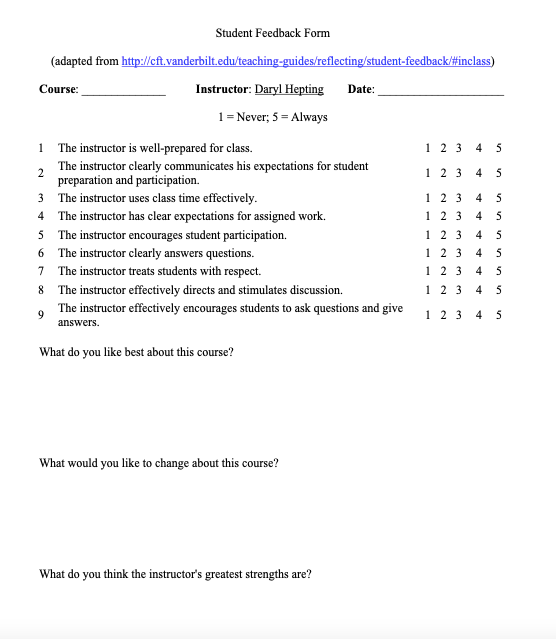
\includegraphics[width=15cm]{images/ch4/Figure2.png}
    \caption{The Student Feedback Form, from Hepting~\cite{prof}}
    \label{fig:4.2}
\end{figure}
\par To commence with the process of building the survey ontology, a new project needs to be created with a unique \ac{iri}\footnote{https://www.w3.org/2011/rdf-wg/wiki/IRIs/RDFConceptsProposal}  and the ontology version. Figure~\ref{fig:4.3} shows the Protégé home-screen with a new project created and an \ac{iri} with the name and version of ontology.
\begin{figure}[htp]
    \centering
    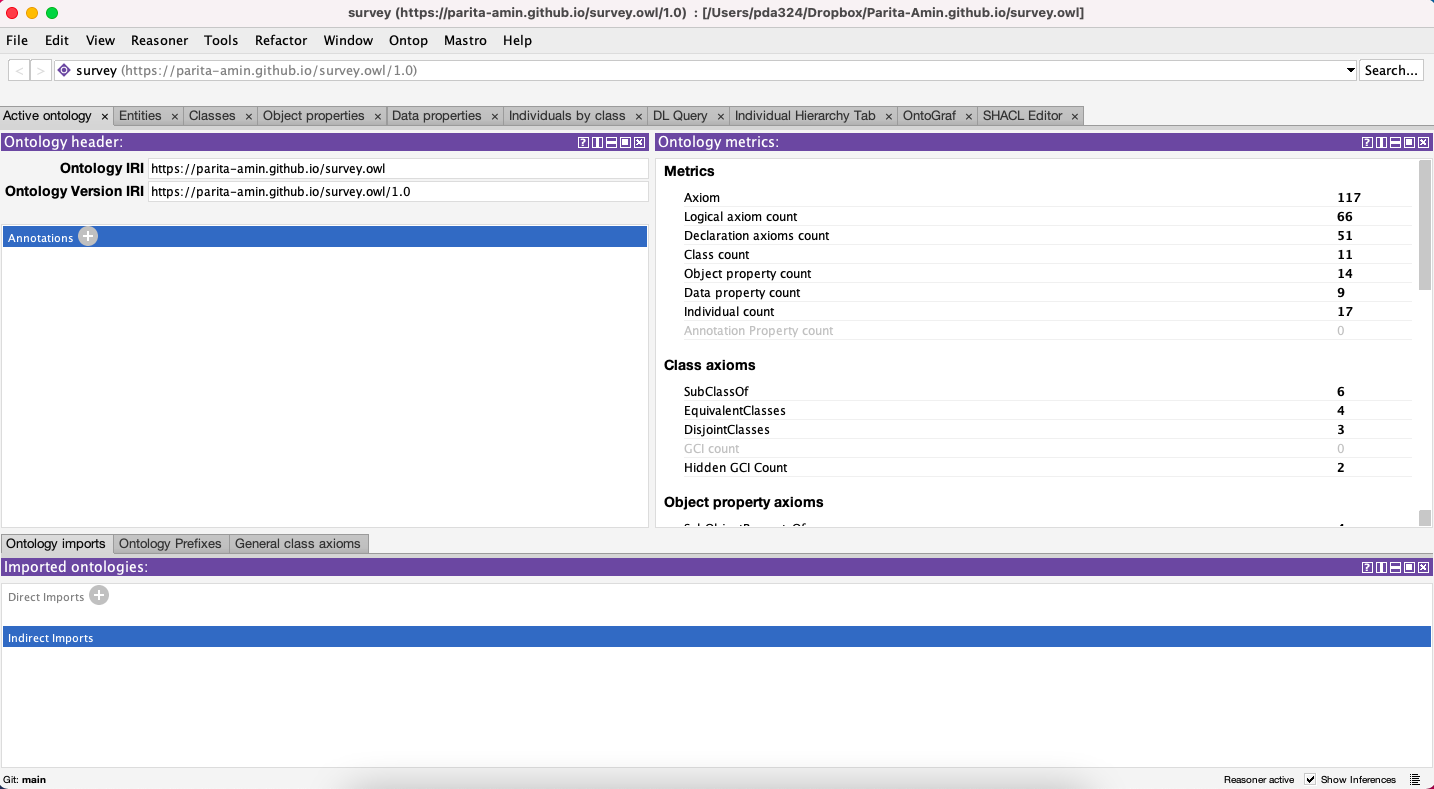
\includegraphics[width=15cm]{images/ch4/Figure3.png}
    \caption{Protégé Home-screen for a New Project with an Ontology Name and an IRI}
    \label{fig:4.3}
\end{figure}
\subsection{Classes and Class Hierarchy}
\par The next step is to create classes and build the hierarchy for the class nodes. Each entity in Protégé is directly or indirectly a child node of the \say{Thing} class. Also, each object has a name-value pair, which generally are the nodes of the \say{Domain\_Entity} class, an inherited class of Thing. Initially, four classes, \say{Thing}, \say{Domain\_Entity}, \say{Independent\_Entity}, and \say{Value} are created using class hierarchy, as shown in Figure~\ref{fig:4.4}. To create a class hierarchy for the classes that represent entities in the survey, there are three steps to be followed:
\begin{figure}[htp]
    \centering
    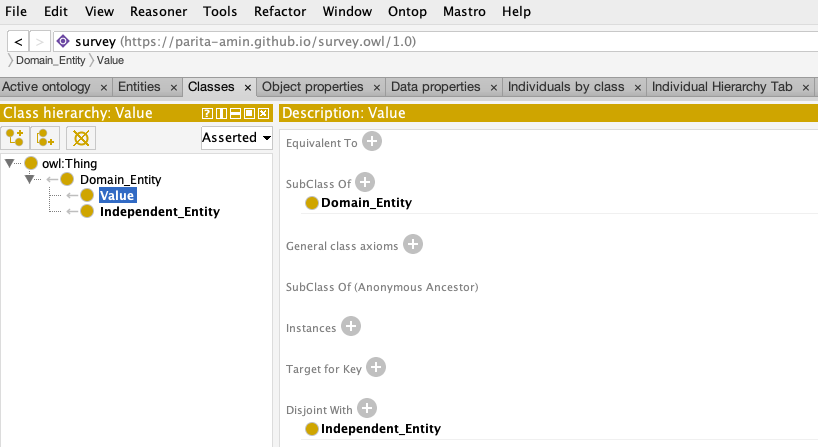
\includegraphics[width=15cm]{images/ch4/Figure4.png}
    \caption{Class Hierarchy of Thing, Domain\_Entity, Independent\_Entity, and Value}
    \label{fig:4.4}
\end{figure}
\begin{enumerate}
    \item Select \say{owl:Thing} in the Class Hierarchy View of the Classes tab from the Windows menu followed by selecting \say{Create class hierarchy...} from the Tools menu, as shown in Figure~\ref{fig:4.5} to open a \say{Enter hierarchy} pop-up window which allows the users to add classes to the ontology.
    \begin{figure}[htp]
    \centering
    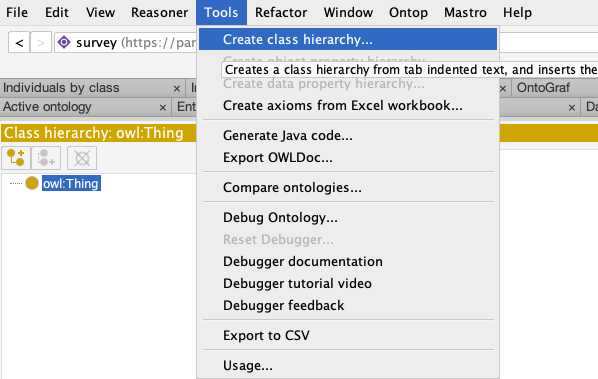
\includegraphics[width=15cm]{images/ch4/Figure5.png}
    \caption{Tools Menu to Create Class Hierarchy}
    \label{fig:4.5}
\end{figure}
    \item Enter the class names in the pop-up window starting from the left. For the child nodes, leave some spaces before writing the class name. Each horizontal line consists of one class name, as shown in Figure~\ref{fig:4.6}. 
    \begin{figure}[htp]
    \centering
    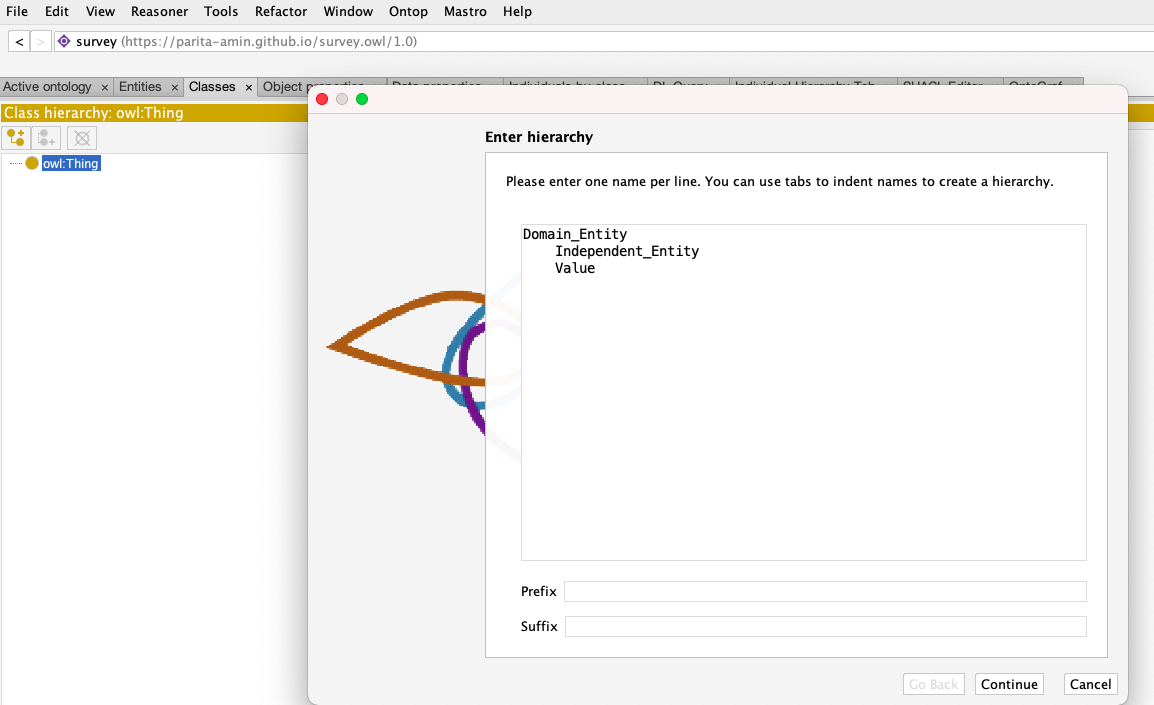
\includegraphics[width=15cm]{images/ch4/Figure6.png}
    \caption{\enquote{Enter hierarchy} Pop-up Window}
    \label{fig:4.6}
\end{figure}
    \item On clicking \say{Continue} on the pop-up window in Figure~\ref{fig:4.6}, it opens up a new pop-up window. Here, it is important to state whether one wants the sibling classes to be disjoint or not. The checkbox needs to be checked accordingly. Usually, it is recommended to create disjoint sibling classes which can be changed later as necessary, as shown in Figure~\ref{fig:4.7}.
    \begin{figure}[htp]
    \centering
    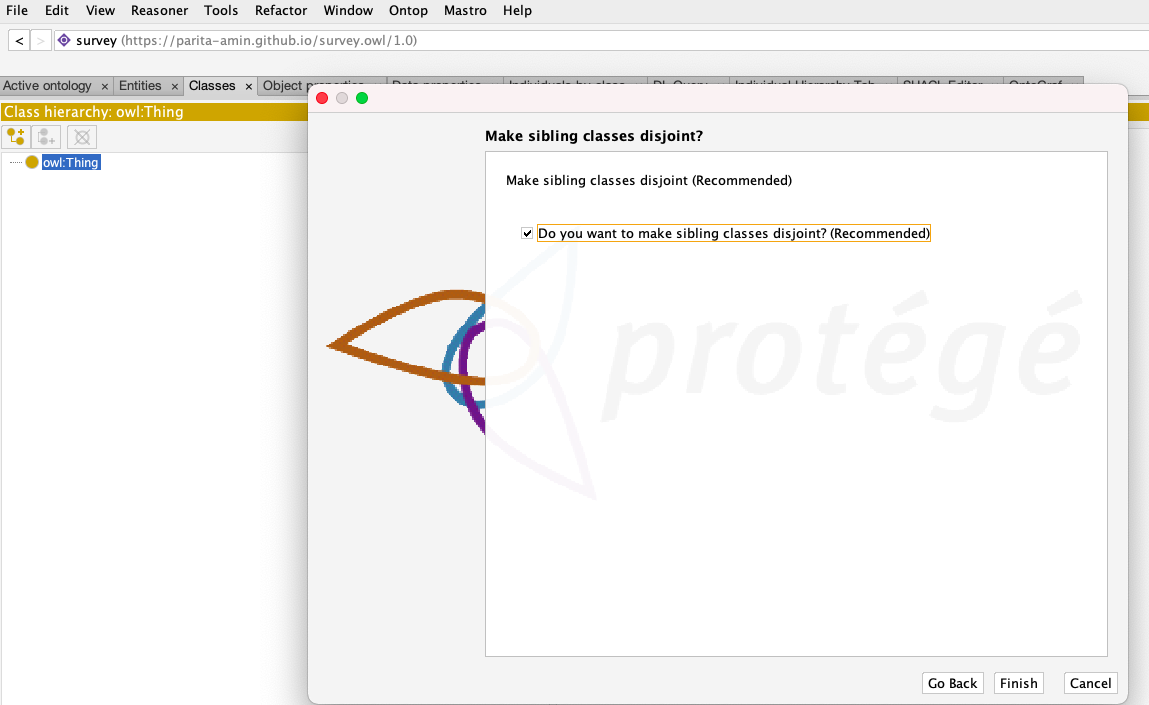
\includegraphics[width=15cm]{images/ch4/Figure7.png}
    \caption{Pop-up Window to Create Disjoint Sibling Classes}
    \label{fig:4.7}
\end{figure}
\end{enumerate}
\par Once the classes are added, the next step is to describe the classes. Descriptions of classes like \say{Equivalent to}, \say{SubClass Of}, \say{Instances}, \say{Disjoint With} and so on can be added using the Description view of the Class tab (shown in Figure~\ref{fig:4.4}). Each class can be described individually by selecting a particular class and adding details to the description view. 
\par All the classes can be created and described using the above steps. In the end, the class hierarchy for the survey ontology would be as shown in Figure~\ref{fig:4.8}. The survey can have \say{Respondent}, \say{Response Date}, \say{Type of Survey}, \say{Survey Questions}, \say{Survey Answers}, and \say{Likert Scale}, which are considered for this ontology as well. Here, the type of survey used is \say{feedback survey}. The survey questions and survey answers would further have entities corresponding to various forms of question-answer. Generally, feedback surveys consist of two types of questions, namely, \say{Likert Questions} and \say{Open-ended Questions}. The type of questions might differ depending on the designer of the survey, some of which, as stated on the \emph{SurveyMonkey}\footnote{https://www.surveymonkey.com/mp/survey-question-types/} website, are listed below. 
\begin{figure}[htp]
    \centering
    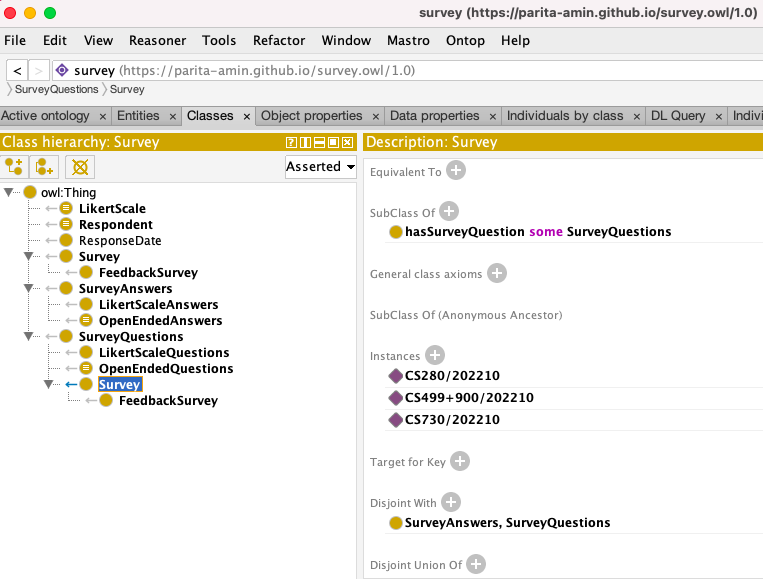
\includegraphics[width=15cm]{images/ch4/Figure8.png}
    \caption{Class Hierarchy in Survey Ontology}
    \label{fig:4.8}
\end{figure}
\begin{multicols}{2}
\begin{itemize}
    \item Multiple Choice Questions
    \item Rating Scale Questions
    \item Likert Scale Questions
    \item Matrix Questions
    \item Dropdown Questions
    \item Open-ended Questions
    \item Demographic Questions
    \item Ranking Questions
    \item Image Choice Questions
    \item Click Map Questions
    \item File Upload Questions
    \item Slider Questions
    \item Benchmarkable Questions
\end{itemize}
\end{multicols}
\par For this research, the feedback survey that has been considered has Likert and Open-ended questions. The entities described for the questions and answers are \say{LikertScaleQuestions}, and \say{OpenEndedQuestions} as sub-classes of \say{SurveyQuestions}, and \say{LikertScaleAnswers}, and \say{OpenEndedAnswers} as sub-classes of \say{SurveyAnswers}.
\par For all the survey questions, there would be a question and an answer, where both of them would be considered as distinct entities. Likert questions are the questions for which the answers are from the preset list of answers. For the Likert questions, the questions can be either of type \say{Never-Always-4} or \say{Never-Always-5} or \say{Never-Always-7} or \say{Never-Always-*}, of which Never-Always-5 has been used by Hepting~\cite{prof}. In a Never-Always-5 type of survey, 5 degrees of agreement are used as shown in Table~\ref{table:4.1}. In addition to these degrees, this ontology also considers the instances where the question wouldn't be answered. In this case, the field corresponding to the answer is left blank. On the other hand, Open-ended questions have unpredictable answers and hence there cannot be any degree of measurement for Open-ended questions.
\begin{table}[h!]
    \centering
    \begin{tabular}{|c|l|}
    \hline Number \ & Agreement \\ \hline
     1 & Never\\ \hline
     2 & [Rarely]\\ \hline
     3 & [Sometimes]\\ \hline
     4 & [Often]\\ \hline
     5 & Always\\ \hline
    \end{tabular}
    \caption{Degrees of Agreement for Likert-scale Questions}
    \label{table:4.1}
\end{table}
\subsection{Object Properties and Object Property Hierarchy}
\par The next step in building the ontology, after describing the classes, is describing the \say{Object Properties}. Object properties are used to link the entities (classes in Protégé). The \say{owl:topObjectProperty} is the root node of the object properties' hierarchy. The hierarchy for object properties can be built by selecting a property in the Object Property Hierarchy view of the Object Property Views tab and then going to the tools menu as shown in Figure~\ref{fig:4.9}. The remaining steps are similar to the ones that are followed for building class hierarchy (Figure~\ref{fig:4.5}, ~\ref{fig:4.6}, and ~\ref{fig:4.7}).
\begin{figure}[htp]
    \centering
    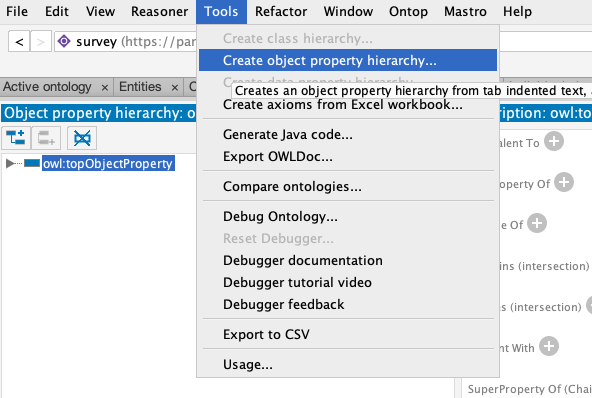
\includegraphics[width=15cm]{images/ch4/Figure9.png}
    \caption{Tools Menu to Create Object Property Hierarchy}
    \label{fig:4.9}
\end{figure}
\par Also, the description view of object properties hierarchy allows the user to describe the object properties. The details that can be added or modified using the description view are \say{Equivalent To}, \say{SubProperty Of}, \say{Inverse Of}, \say{Domains (intersection)}, \say{Ranges (intersection)}, \say{Disjoint With}, and \say{SuperProperty Of (Chain)}. 
\par The names of the object properties usually start with an \say{is} or a \say{has}. For instance, consider two classes: \say{Lady} (class 1) and \say{Parita} (class 2). To describe the link between class 1 (Lady) and class 2 (Parita) such that class 1 has value class 2 and class 2 is value of class 1, the properties \say{hasName} and \say{isNameOf} would be used respectively, as shown in Figure~\ref{fig:4.10}. 
\begin{figure}[htp]
    \centering
    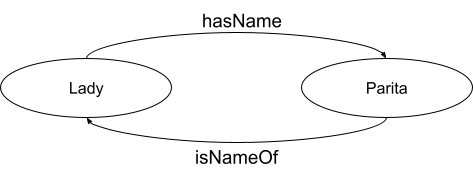
\includegraphics[width=15cm]{images/ch4/Figure10.png}
    \caption{Object Properties for Classes \enquote{Lady} and \enquote{Parita}}
    \label{fig:4.10}
\end{figure}
\par Each object property might have a corresponding inverse property. For the above instance, it can be said that:
\begin{center}
    \par Lady hasName Parita \textbf{is equivalent to} Parita isNameOf Lady
\end{center}
Here, \say{hasName} is inverse of \say{isNameOf} and \say{isNameOf} is inverse of \say{hasName}. Apart from inverse, domain and range\footnote{http://protegeproject.github.io/protege/views/object-property-description/} are two other important parts of description of object properties. According to Horridge et al.~\cite{horridge2009practical}, in \ac{owl}, \say{domain and range are not constraints to be checked. They are axioms which are used by the reasoner to make inferences}. As shown in Figure~\ref{fig:4.11}, \say{Lady} acts as the \say{Domain} and \say{Parita} acts as the \say{Range} for \say{hasName} whereas for \say{isNameOf}, \say{Parita} is the \say{Domain} and \say{Lady} is the \say{Range}. 
\begin{figure}[htp]
    \centering
    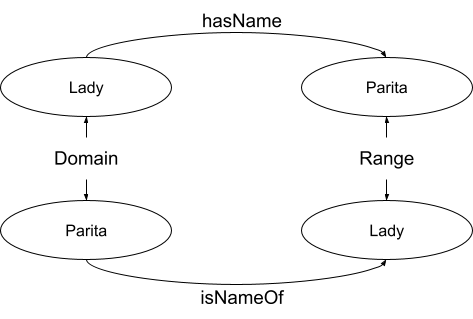
\includegraphics[width=12cm]{images/ch4/Figure11.png}
    \caption{Domain and Range Classes for \enquote{hasName} and \enquote{isNameOf}}
    \label{fig:4.11}
\end{figure}
\par Using the above method of naming and building object properties, some of the primary object properties are described for the survey ontology as shown in Figure~\ref{fig:4.12} where as Table~\ref{table:4.2} shows the list of the object properties along with their domain and range classes (entities). Table~\ref{table:4.3} consists of the parent nodes and inverse properties of the object properties. The three parent nodes involved in object property hierarchy are \say{owl:TopObjectProperty}, \say{hasContent}, and \say{isContentOf}. Protégé has a built-in \say{Reasoner} that allows the users to determine inconsistencies of a class as well as to discover implicit information.
\begin{figure}[htp]
    \centering
    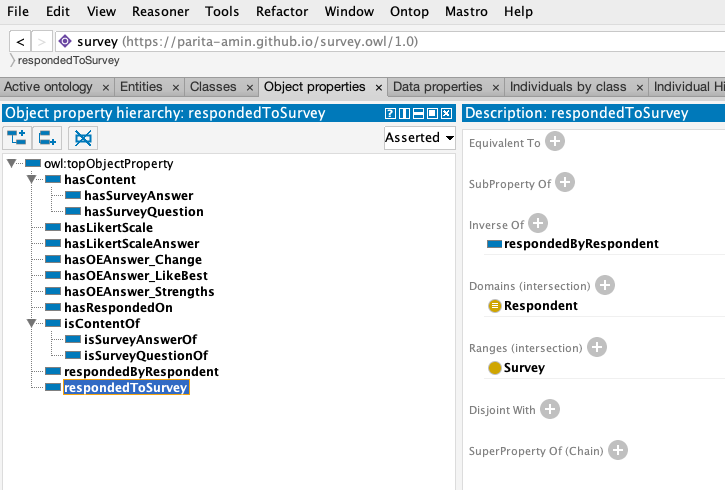
\includegraphics[width=15cm]{images/ch4/Figure12.png}
    \caption{Object Property Hierarchies, Domain and Range for Classes}
    \label{fig:4.12}
\end{figure}
\begin{table}[h!]
    \centering
    \begin{tabular}{|l|l|l|} 
    \hline Object Property & Domain & Range\\ \hline
     hasSurveyQuestion & Survey & SurveyQuestions\\ \hline
     hasLikertScale & LikertScaleQuestions & LikertScale\\ \hline
     hasLikertScaleAnswer & Respondent & LikertScale\\ \hline
     hasRespondedOn & Respondent & ResponseDate\\ \hline
     respondedToSurvey & Respondent & Survey\\ \hline
     hasOEAnswer\_Change & OpenEndedQuestions & OpenEndedAnswers\\ \hline
     hasOEAnswer\_LikeBest & OpenEndedQuestions & OpenEndedAnswers\\ \hline
     hasOEAnswer\_Strengths & OpenEndedQuestions & OpenEndedAnswers\\ \hline
    \end{tabular}
    \caption{Object Properties and Their Domain and Range}
    \label{table:4.2}
    \end{table}
\begin{table}[h!]
    \centering
    \begin{tabular}{|l|l|l|} 
    \hline Object Property & Parent Node & Inverse Property\\ \hline
     hasContent & owl:TopObjectProperty & isContentOf\\ \hline
     isContentOf & owl:TopObjectProperty & hasContent\\ \hline
     hasLikertScale & owl:TopObjectProperty & \\ \hline
     hasLikertScaleAnswer & owl:TopObjectProperty & \\ \hline
     hasOEAnswer\_Change & owl:TopObjectProperty & \\ \hline
     hasOEAnswer\_LikeBest & owl:TopObjectProperty & \\ \hline
     hasOEAnswer\_Strengths & owl:TopObjectProperty & \\ \hline
     hasRespondedOn & owl:TopObjectProperty & \\ \hline
     respondedByRespondent & owl:TopObjectProperty & respondedToSurvey\\ \hline
     respondedToSurvey & owl:TopObjectProperty & respondedByRespondent\\ \hline
     hasSurveyQuestion & hasContent & isSurveyQuestionOf\\ \hline
     hasSurveyAnswer & hasContent & isSurveyAnswerOf\\ \hline
     isSurveyQuestionOf & isContentOf & hasSurveyQuestion\\ \hline
     isSurveyAnswerOf & isContentOf & hasSurveyAnswer\\ \hline
    \end{tabular}
    \caption{Object Properties with Their Parent Nodes and Inverse Properties}
    \label{table:4.3}
    \end{table}
\subsection{Data Properties and Data Property Hierarchy}
\par Furthermore, the \say{Data Properties} can also be described for ontology. \say{An ontology data property provides a relation to attach an entity instance to some literal datatype value (an \ac{rdf} number, string or data for example) that is a measure or estimate of what that data property is about.}\footnote{https://ddooley.github.io/docs/data-properties/} In Protégé, the \say{owl:topDataProperty} is the root node of the data properties' hierarchy. The data property hierarchy can be built by selecting a property in the Data Property Hierarchy view of the Data Property Views tab and then going to the tools menu as shown in Figure~\ref{fig:4.13}. The remaining steps are similar to the ones that are followed for building class and object property hierarchy (Figure~\ref{fig:4.5}, ~\ref{fig:4.6}, and ~\ref{fig:4.7}). 
\begin{figure}[htp]
    \centering
    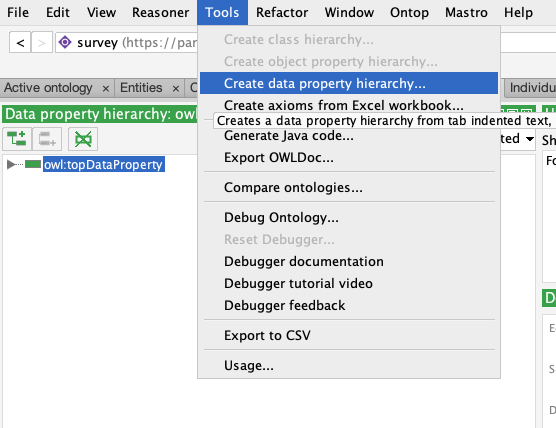
\includegraphics[width=15cm]{images/ch4/Figure13.png}
    \caption{Tools Menu to Create Data Property Hierarchy}
    \label{fig:4.13}
\end{figure}
\par Data properties can be described using the description view of data properties of hierarchy which included details like \say{Equivalent To}, \say{SubProperty Of}, \say{Domains (intersection)}, \say{Ranges}, and  \say{Disjoint With}. Figure~\ref{fig:4.14} shows the data properties described for the survey ontology. The parent node of all the data properties is \say{owl:topDataProperty} and the domain and range for all the data properties are \say{Respondent} and \say{xsd:positiveInteger} respectively. Table~\ref{table:4.4} consists of list of data properties along with their domain and range classes (entities).
\begin{figure}[htp]
    \centering
    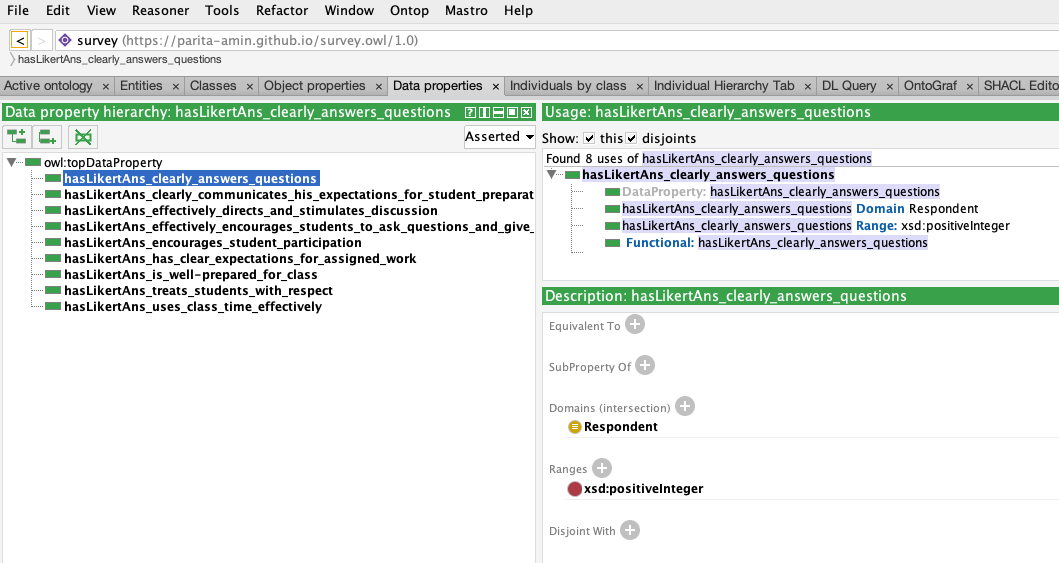
\includegraphics[width=15cm]{images/ch4/Figure14.png}
    \caption{Data Property Hierarchies, Domain and Range for Classes}
    \label{fig:4.14}
\end{figure}
\begin{table}[h!]
    \centering
    \begin{tabular}{|l|l|l|} 
    \hline \ \ \ \ \ \ \ \ \ \ \ \ \ \ \ Data Property &\ Domain &\ \ \ \ \ \ \ Range\\ \hline
     hasLikertAns\_is\_well-prepared\_for&\\ \_class & \multirow{-2}{5em}{Respondent} & \multirow{-2}{8.5em}{xsd:positiveInteger}\\ \hline
     hasLikertAns\_clearly\_communicates&\\ \_his\_expectations\_for\_student&\\ \_preparation\_and\_participation & \multirow{-3}{5em}{Respondent} & \multirow{-3}{8.5em}{xsd:positiveInteger}\\ \hline
     hasLikertAns\_uses\_class\_time&\\ \_effectively & \multirow{-2}{5em}{Respondent} & \multirow{-2}{8.5em}{xsd:positiveInteger}\\ \hline
     hasLikertAns\_has\_clear\_expectations&\\ \_for\_assigned\_work & \multirow{-2}{5em}{Respondent} & \multirow{-2}{8.5em}{xsd:positiveInteger}\\ \hline
     hasLikertAns\_encourages\_student&\\ \_participation & \multirow{-2}{5em}{Respondent} & \multirow{-2}{8.5em}{xsd:positiveInteger}\\ \hline
     hasLikertAns\_clearly\_answers&\\ \_questions & \multirow{-2}{5em}{Respondent} & \multirow{-2}{8.5em}{xsd:positiveInteger}\\ \hline
     hasLikertAns\_treats\_students&\\ \_with\_respect & \multirow{-2}{5em}{Respondent} & \multirow{-2}{8.5em}{xsd:positiveInteger}\\ \hline
     hasLikertAns\_effectively\_directs&\\ \_and\_stimulates\_discussion & \multirow{-2}{5em}{Respondent} & \multirow{-2}{8.5em}{xsd:positiveInteger}\\ \hline
     hasLikertAns\_effectively\_encourages&\\ \_students\_to\_ask\_questions\_and&\\ \_give\_answers & \multirow{-3}{5em}{Respondent} & \multirow{-3}{8.5em}{xsd:positiveInteger}\\ \hline
    \end{tabular}
    \caption{Data Properties and Their Domain and Range}
    \label{table:4.4}
    \end{table}
\subsection{Individuals}
\par 
\par After describing the classes, object properties, data properties, and individuals, the next step is to determine and fix the errors and inconsistencies in the ontology using a Reasoner. The final class hierarchy of the \ac{owl} ontology in Protégé, after using the HermiT 1.4.3.456 reasoner, would be as shown in Figure~\ref{fig:4.15}.
\begin{figure}[htp]
    \centering
    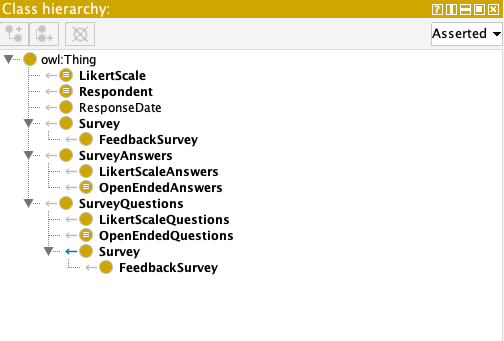
\includegraphics[width=15cm]{images/ch4/Figure15.png}
    \caption{Class Hierarchy for the Final Version of Survey Ontology}
    \label{fig:4.15}
\end{figure}
\par The grey (all entities) and blue (\say{Survey} entity) back arrows in front of the yellow solid dot, which indicates class, show parent/child relationship other than that of SubClassOf. This feature can be enabled and disabled by selecting \say{Display relationship in class hierarchy} option from the \say{View} menu of Protégé. Figure~\ref{fig:4.16} shows the relation indicated by the blue back arrow.
\begin{figure}[htp]
    \centering
    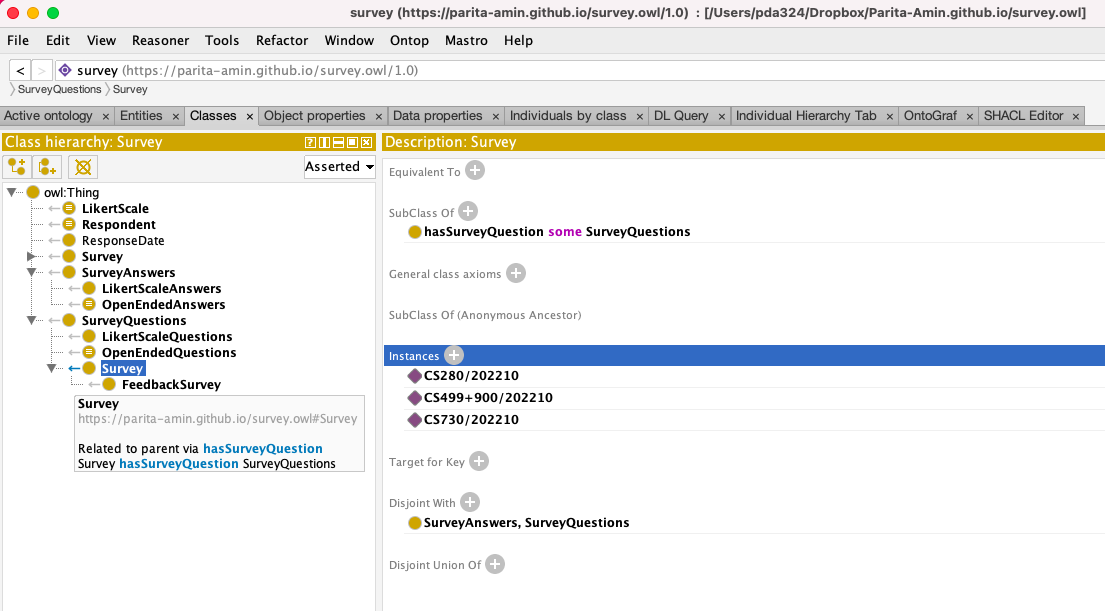
\includegraphics[width=15cm]{images/ch4/Figure16.png}
    \caption{Parent/Child Relation indicated by "Blue Back" Arrow}
    \label{fig:4.16}
\end{figure}
\section{Visualization Tools for \ac{owl} Ontology}
\par The next step is visualization of the built \ac{owl} ontology using various visualization tools. Protégé supports plug-ins for some visualization tools like OntoGraf and \ac{owl}Viz whereas tools like WebVOWL, RelFinder and \ac{owl}GrEd are available for use as web-based tools. This section focuses on the two tools, OntoGraf and WebVOWL, used for the visualization of the survey ontology in this research.
\subsection{OntoGraf}
\par Falconer~\cite{falconer2010ontograf} introduced OntoGraf as a Protégé plug-in for the visualization of the \ac{owl} ontologies. This tool helps the users to represent the ontologies, built using Protégé, by repetitively allowing and restricting the desired classes. OntoGraf offers various graph layout options for visualization like Grid Layout\footnote{classes are arranged in a grid alphabetically}, Spring Layout, and Tree Layout\footnote{both horizontal and vertical}. Antoniazzi and Viola~\cite{antoniazz2018rdf} stated that the \say{individuals of a class can be visualized in its tooltip, but this is uncomfortable when dealing with a high number of assertional statements}. The graphs generated using OntoGraf can be exported as image files of various formats such as \ac{png}, \ac{jpeg}, \ac{gif} and as a dot file\footnote{a Microsoft Word Template with the details of default settings}.
\par Figure~\ref{fig:4.17} shows the graph generated using OntoGraf for the survey ontology. To start with the graph formation, the classes \say{Thing}, \say{Domain\_entity}, \say{Independent\_entity} and \say{Value} were selected followed by expansion of \say{Independent\_entity} and \say{Value} classes by double-clicking them. This expansion adds all the classes that are connected to the classes. The classes connected includes both the subclasses as well as the ones linked through the object properties. Solid blue lines are used to denote the relationships between the classes and their subclasses whereas dashed lines are used to represent the object properties.
\begin{figure}[htp]
    \centering
    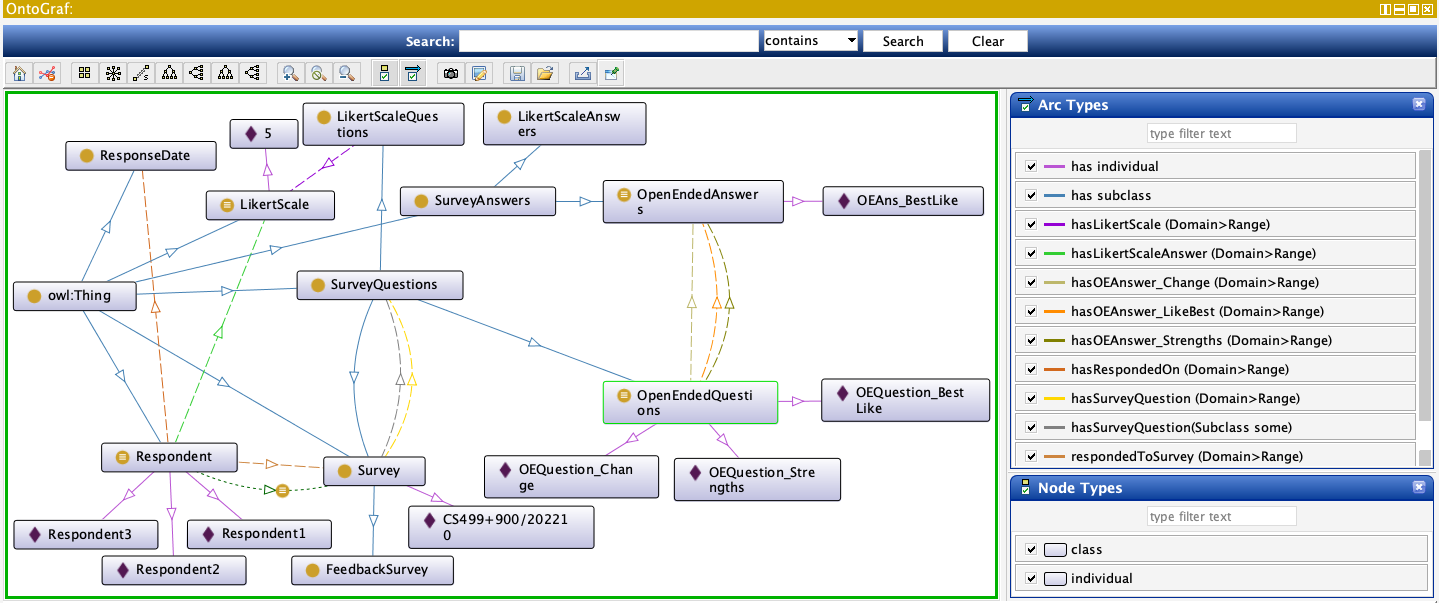
\includegraphics[width=15cm]{images/ch4/Figure17.png}
    \caption{OntoGraf for Survey Ontology}
    \label{fig:4.17}
\end{figure}
\subsection{WebVOWL}
\par WebVOWL~\cite{lohmann2014webvowl}, the Web-based \ac{vowl}, one of the variety of forms in which the \ac{vowl} visualization tool is available, represents the \say{ontologies graphically using a force-directed graph layout}~\cite{antoniazz2018rdf}. \ac{vowl} follows some ground rules for the representation of \ac{owl} ontologies which are:
\begin{enumerate}
    \item Circles are used to denote classes. Also, different types are assigned different colors. For instance, \ac{owl} classes are denoted using \say{light blue circles}.
    \item Black solid lines are used to represent \ac{owl} object and datatype properties. The object properties use light blue labels where as the datatype properties are labelled in green.
    \item The relationships between the classes and their subclasses are represented using dashed lines.
\end{enumerate}
\par Figure~\ref{fig:4.18} shows the graphical representation of the survey ontology using Web\ac{vowl}. The figure focuses on only some of the class-subclass relationships and some of the object properties. The metadata and the statistics of the node (circle) or the edge (line) can be retrieved by clicked on them. The entities (classes) and their relationships (object and datatype properties) can be presented or restricted using filters. The \ac{vowl} graph can be exported as an \ac{svg} image file or a \ac{json} code file.
\begin{figure}[htp]
    \centering
    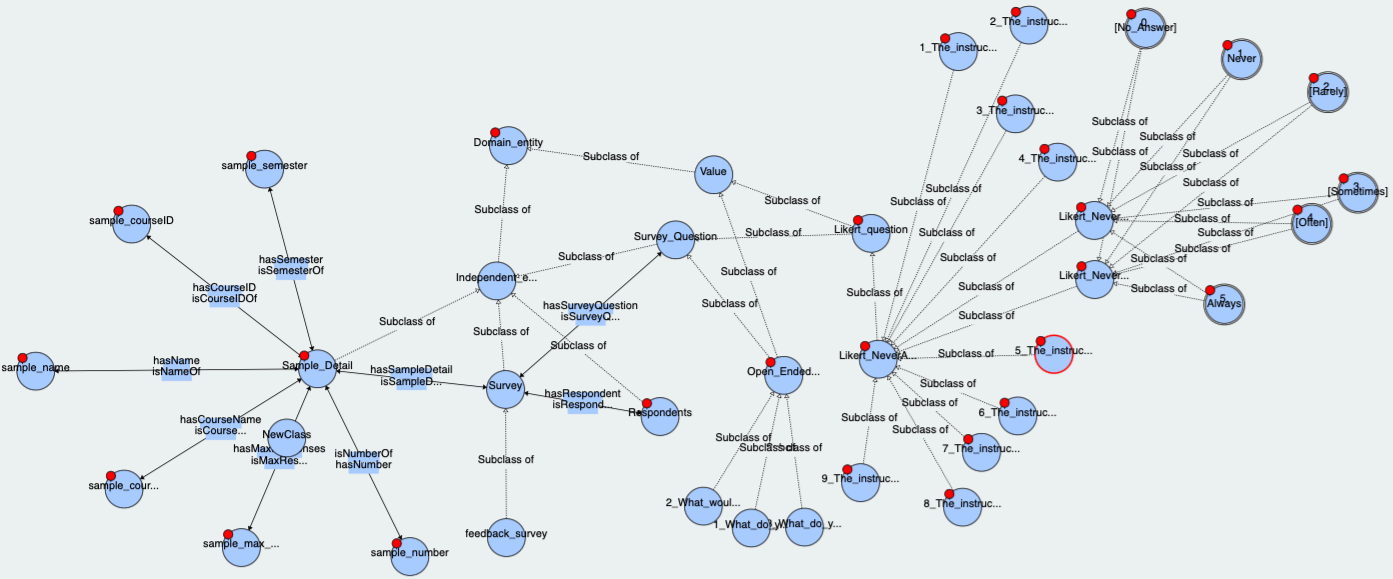
\includegraphics[width=15.5cm]{images/ch4/Figure18.png}
    \caption{WebVOWL for Survey Ontology}
    \label{fig:4.18}
\end{figure}
\end{doublespace}
%!TEX root = parita-msc.tex

\chapter{Conclusion and Future Work}
\label{chap:conclusion}
\begin{doublespace}
This Chapter focuses on the prime offerings of this research work where one of the sections includes the conclusions drawn from the work done and the other discusses future work that can be done to succeed in this research.
\section{Conclusion}
\par This thesis work describes a new attempt on developing a linked open data instrument for feedback surveys. It focuses on the issues encountered and the user experience of various tools and references used for the modelling of the instrument and for data visualization. The thesis revolves around some fundamental topics like Semantic Web, Linked Open Data, \ac{rdf}, and \ac{owl} ontologies. It also describes how and why Protégé has been used over other ontology development tools to describe survey vocabularies. The thesis can be considered as a guide for the researchers who are interested in exploring this lesser known aspect of semantic web.
\par The thesis includes a detailed background study on the fundamental topics, the usability of Protégé, and discussion on some tools for linked open data visualizations. Chapter~\ref{chap:ontology} describes the steps involved in building the survey ontology using Protégé, various parts and facilities offered by Protégé, and the visual representation of the ontology toward the end.
\section{Future Work}
%\par A new aspect opens a wide range of future opportunities for the researchers to work upon. 
\par This thesis also offers a number of future development options like building a real-time linked open data application for feedback surveys that 
%obeys 
follows the linked data life cycle. 
%The current research mentions a list of vocabularies which can be defined with detailed properties and published on one of the open platforms. 
Web Scraping (or Web Extraction) is a method of extracting desired data from the resources on the \ac{www} into a separate file for data retrieval and data analysis. Data Extraction is one of the steps in the linked data life cycle that can be explored in future research to facilitate use of data that has already been published to the web with HTML tables.
\par Versioning of the survey ontology is a topic of interest. The ontology vocabularies (available in Appendix~\ref{chap:appendix3}) can be reused for appropriate applications but they may need to be updated over time.
%as the vocabularies are not static. The existing vocabularies might not be specific to a particular purpose. 
Hence, ontology versioning and version management of the survey instrument for this feedback survey,
as well as for other types of surveys is an aspect of this research that can be explored.
\par Developing a data entry form for the feedback survey instrument
that can be defined, in part, directly from the survey ontology would facilitate recording of survey responses collected offline.
%can also be added to the list of future works. A data entry form depending on the data required by the survey instrument can be developed which facilitates entering and recording the responses collected for the survey.

 \end{doublespace}

\appendix
%!TEX root = parita-msc.tex

\chapter{Sample CSV Data}
\label{chap:appendix1}
\begin{doublespace}
\begin{lstlisting}
Likert Item,5 Always,4 [Mostly],3 [Sometimes],2 [Rarely],1 Never,Total
1. The instructor is well-prepared for class,29,16,8,0,0,53
2. The instructor clearly communicates his expectations for student 
    preparation and participation,33,15,4,1,0,53
3. The instructor uses class time effectively,26,18,7,2,0,53
4. The instructor has clear expectations for assigned work,34,10,8,1,0,53
5. The instructor encourages student participation,45,6,2,0,0,53
6. The instructor clearly answers questions,31,16,5,1,0,53
7. The instructor treats students with respect,49,3,1,0,0,53
8. The instructor effectively directs and stimulates discussion,
    38,10,4,1,0,53
9. The instructor effectively encourages students to ask questions and 
    give answers,43,8,2,0,0,53
Total,328,102,41,6,0,477
Weighted Average: 91% 'Always'
Response,Q1,Q2,Q3,Q4,Q5,Q6,Q7,Q8,Q9,Avg,SD,Mode,Median
1,5,5,5,5,5,5,5,5,5,5.00,0.00,5,5
2,4,3,3,2,3,4,5,3,4,3.44,0.88,3,3
3,5,5,5,5,5,5,5,5,5,5.00,0.00,5,5
4,5,5,4,5,5,5,5,5,5,4.89,0.33,5,5
5,5,5,4,5,5,5,5,4,5,4.78,0.44,5,5
6,3,4,4,3,5,4,5,5,5,4.22,0.83,5,4
7,3,4,4,4,4,4,5,3,3,3.78,0.67,4,4
8,4,4,4,4,5,5,5,5,5,4.56,0.53,5,5
9,5,5,5,5,5,5,5,5,5,5.00,0.00,5,5
10,4,5,4,5,5,5,4,4,5,4.56,0.53,5,5
11,5,5,5,5,5,5,5,5,5,5.00,0.00,5,5
12,5,5,5,4,5,4,5,5,5,4.78,0.44,5,5
13,5,5,5,5,5,5,5,5,5,5.00,0.00,5,5
14,5,5,5,5,5,5,5,5,5,5.00,0.00,5,5
15,4,5,4,4,5,5,5,5,5,4.67,0.50,5,5
16,5,5,4,5,5,5,5,5,5,4.89,0.33,5,5
17,5,5,5,5,5,5,5,5,5,5.00,0.00,5,5
18,3,4,5,3,3,2,3,4,4,3.44,0.88,3,3
19,3,3,3,3,5,3,5,4,5,3.78,0.97,3,3
20,4,4,4,5,5,5,5,5,5,4.67,0.50,5,5
21,4,4,3,5,5,4,5,5,5,4.44,0.73,5,5
22,3,3,3,3,5,3,5,4,5,3.78,0.97,3,3
23,4,4,4,3,5,4,5,5,5,4.33,0.71,4,4
24,4,4,5,5,5,4,5,5,5,4.67,0.50,5,5
25,3,2,2,3,4,3,5,3,4,3.22,0.97,3,3
26,3,3,2,3,4,3,4,2,3,3.00,0.71,3,3
27,5,5,4,5,5,5,5,4,4,4.67,0.50,5,5
28,5,5,5,5,5,5,5,5,5,5.00,0.00,5,5
29,4,4,4,3,5,4,5,5,4,4.22,0.67,4,4
30,4,5,4,5,5,4,5,5,4,4.56,0.53,5,5
31,5,5,5,5,5,4,5,5,5,4.89,0.33,5,5
32,5,5,5,5,4,5,5,4,5,4.78,0.44,5,5
33,5,5,5,5,5,5,5,5,5,5.00,0.00,5,5
34,5,5,5,5,5,5,5,5,5,5.00,0.00,5,5
35,5,5,5,5,5,5,5,5,5,5.00,0.00,5,5
36,4,4,3,4,5,5,5,5,5,4.44,0.73,5,5
37,5,5,5,5,5,5,5,4,5,4.89,0.33,5,5
38,4,4,3,4,5,3,5,4,5,4.11,0.78,4,4
39,5,5,5,4,5,4,5,5,4,4.67,0.50,5,5
40,5,5,5,5,5,5,5,5,5,5.00,0.00,5,5
41,5,4,5,5,5,5,5,5,5,4.89,0.33,5,5
42,5,5,5,5,5,5,5,5,5,5.00,0.00,5,5
43,4,5,4,5,5,5,5,5,5,4.78,0.44,5,5
44,4,5,4,5,4,4,5,4,5,4.44,0.53,4,4
45,5,5,5,5,5,5,5,5,5,5.00,0.00,5,5
46,3,4,4,4,4,4,5,3,4,3.89,0.60,4,4
47,5,5,5,5,5,5,5,5,5,5.00,0.00,5,5
48,4,4,4,5,5,4,4,5,5,4.44,0.53,4,4
49,4,4,3,4,5,5,5,5,5,4.44,0.73,5,5
50,5,5,4,4,5,4,5,5,5,4.67,0.50,5,5
51,5,5,5,5,5,5,5,5,5,5.00,0.00,5,5
52,5,5,5,5,5,5,5,5,5,5.00,0.00,5,5
53,5,5,5,5,5,4,5,5,5,4.89,0.33,5,5
Avg,4.40,4.51,4.28,4.45,4.81,4.45,4.91,4.60,4.77,4.58,0.21
SD,0.74,0.72,0.84,0.82,0.48,0.75,0.35,0.72,0.51
Mode,5,5,5,5,5,5,5,5,5
Median,5,5,4,5,5,5,5,5,5
\end{lstlisting}
\end{doublespace}

%!TEX root = parita-msc.tex

\chapter{Expression of CSV Data in RDF}
\label{chap:appendix2}
%\begin{doublespace}
\lstset{ 
  %backgroundcolor=\color{white},   % choose the background color; you must add \usepackage{color} or \usepackage{xcolor}; should come as last argument
  basicstyle=\footnotesize,        % the size of the fonts that are used for the code
  breakatwhitespace=false,         % sets if automatic breaks should only happen at whitespace
  breaklines=true,                 % sets automatic line breaking
  captionpos=b,                    % sets the caption-position to bottom
  %commentstyle=\color{mygreen},    % comment style
  %deletekeywords={...},            % if you want to delete keywords from the given language
  escapeinside={\%*}{*)},          % if you want to add LaTeX within your code
  %extendedchars=true,              % lets you use non-ASCII characters; for 8-bits encodings only, does not work with UTF-8
  firstnumber=1,                % start line enumeration with line 1000
  %frame=single,	                   % adds a frame around the code
  keepspaces=true,                 % keeps spaces in text, useful for keeping indentation of code (possibly needs columns=flexible)
  %keywordstyle=\color{blue},       % keyword style
  language=XML,                 % the language of the code
  %morekeywords={*,...},            % if you want to add more keywords to the set
  numbers=left,                    % where to put the line-numbers; possible values are (none, left, right)
  numbersep=5pt,                   % how far the line-numbers are from the code
  %numberstyle=\tiny\color{mygray}, % the style that is used for the line-numbers
  %rulecolor=\color{black},         % if not set, the frame-color may be changed on line-breaks within not-black text (e.g. comments (green here))
  showspaces=false,                % show spaces everywhere adding particular underscores; it overrides 'showstringspaces'
  showstringspaces=false,          % underline spaces within strings only
  showtabs=false,                  % show tabs within strings adding particular underscores
  stepnumber=2,                    % the step between two line-numbers. If it's 1, each line will be numbered
  %stringstyle=\color{mymauve},     % string literal style
  tabsize=2,	                   % sets default tabsize to 2 spaces
  title=\lstname                   % show the filename of files included with \lstinputlisting; also try caption instead of title
}
\begin{lstlisting}
<?xml version="1.0" encoding="UTF-8"?>
<rdf:RDF
	xmlns:rdf="http://www.w3.org/1999/02/22-rdf-syntax-ns#"
	xmlns:owl="http://www.w3.org/2002/07/owl#"
	xmlns:rdfs="http://www.w3.org/2000/01/rdf-schema#"
	xmlns:foaf="http://xmlns.com/foaf/0.1/">
<rdf:Description rdf:about="http://survey.org/Question_1.
%20The%20instructor%20is%20well-prepared%20for%20class">
	<Always xmlns="http://survey.org/likert/" rdf:datatype=
	"http://www.w3.org/2001/XMLSchema#int">29</Always>
	<Mostly xmlns="http://survey.org/likert/" rdf:datatype=
	"http://www.w3.org/2001/XMLSchema#int">16</Mostly>
	<Sometimes xmlns="http://survey.org/likert/" rdf:datatype=
	"http://www.w3.org/2001/XMLSchema#int">8</Sometimes>
	<Rarely xmlns="http://survey.org/likert/">0</Rarely>
	<Never xmlns="http://survey.org/likert/">0</Never>
</rdf:Description>

<rdf:Description rdf:about="http://survey.org/likert/Total">
	<Responses xmlns="http://survey.org/likert/" rdf:datatype=
	"http://www.w3.org/2001/XMLSchema#int">53</Responses>
</rdf:Description>

<rdf:Description rdf:about="http://survey.org/Question_2.
%20The%20instructor%20clearly%20communicates%20his%20expectations
%20for%20student%20preparation%20and%
20participation">
	<Always xmlns="http://survey.org/likert/" rdf:datatype=
	"http://www.w3.org/2001/XMLSchema#int">33</Always>
	<Mostly xmlns="http://survey.org/likert/" rdf:datatype=
	"http://www.w3.org/2001/XMLSchema#int">15</Mostly>
	<Sometimes xmlns="http://survey.org/likert/" rdf:datatype=
	"http://www.w3.org/2001/XMLSchema#int">4</Sometimes>
	<Rarely xmlns="http://survey.org/likert/">1</Rarely>
	<Never xmlns="http://survey.org/likert/">0</Never>
</rdf:Description>

<rdf:Description rdf:about="http://survey.org/likert/Total">
	<Responses xmlns="http://survey.org/likert/" rdf:datatype=
	"http://www.w3.org/2001/XMLSchema#int">53</Responses>
</rdf:Description>

<rdf:Description rdf:about="http://survey.org/Question_3.
%20The%20instructor%20uses%20class%20time%20effectively">
	<Always xmlns="http://survey.org/likert/" rdf:datatype=
	"http://www.w3.org/2001/XMLSchema#int">26</Always>
	<Mostly xmlns="http://survey.org/likert/" rdf:datatype=
	"http://www.w3.org/2001/XMLSchema#int">18</Mostly>
	<Sometimes xmlns="http://survey.org/likert/" rdf:datatype=
	"http://www.w3.org/2001/XMLSchema#int">7</Sometimes>
	<Rarely xmlns="http://survey.org/likert/">2</Rarely>
	<Never xmlns="http://survey.org/likert/">0</Never>
</rdf:Description>

<rdf:Description rdf:about="http://survey.org/likert/Total">
	<Responses xmlns="http://survey.org/likert/" rdf:datatype=
	"http://www.w3.org/2001/XMLSchema#int">53</Responses>
</rdf:Description>

<rdf:Description rdf:about="http://survey.org/Question_4.
%20The%20instructor%20has%20clear%20expectations%20for
%20assigned%20work">
	<Always xmlns="http://survey.org/likert/" rdf:datatype=
	"http://www.w3.org/2001/XMLSchema#int">34</Always>
	<Mostly xmlns="http://survey.org/likert/" rdf:datatype=
	"http://www.w3.org/2001/XMLSchema#int">10</Mostly>
	<Sometimes xmlns="http://survey.org/likert/" rdf:datatype=
	"http://www.w3.org/2001/XMLSchema#int">8</Sometimes>
	<Rarely xmlns="http://survey.org/likert/">1</Rarely>
	<Never xmlns="http://survey.org/likert/">0</Never>
</rdf:Description>

<rdf:Description rdf:about="http://survey.org/likert/Total">
	<Responses xmlns="http://survey.org/likert/" rdf:datatype=
	"http://www.w3.org/2001/XMLSchema#int">53</Responses>
</rdf:Description>

<rdf:Description rdf:about="http://survey.org/Question_5.%20The
%20instructor%20encourages%20student%20participation">
	<Always xmlns="http://survey.org/likert/" rdf:datatype=
	"http://www.w3.org/2001/XMLSchema#int">45</Always>
	<Mostly xmlns="http://survey.org/likert/" rdf:datatype=
	"http://www.w3.org/2001/XMLSchema#int">6</Mostly>
	<Sometimes xmlns="http://survey.org/likert/" rdf:datatype=
	"http://www.w3.org/2001/XMLSchema#int">2</Sometimes>
	<Rarely xmlns="http://survey.org/likert/">0</Rarely>
	<Never xmlns="http://survey.org/likert/">0</Never>
</rdf:Description>

<rdf:Description rdf:about="http://survey.org/likert/Total">
	<Responses xmlns="http://survey.org/likert/" rdf:datatype=
	"http://www.w3.org/2001/XMLSchema#int">53</Responses>
</rdf:Description>

<rdf:Description rdf:about="http://survey.org/Question_6.%20The
%20instructor%20clearly%20answers%20questions">
	<Always xmlns="http://survey.org/likert/" rdf:datatype=
	"http://www.w3.org/2001/XMLSchema#int">31</Always>
	<Mostly xmlns="http://survey.org/likert/" rdf:datatype=
	"http://www.w3.org/2001/XMLSchema#int">16</Mostly>
	<Sometimes xmlns="http://survey.org/likert/" rdf:datatype=
	"http://www.w3.org/2001/XMLSchema#int">5</Sometimes>
	<Rarely xmlns="http://survey.org/likert/">1</Rarely>
	<Never xmlns="http://survey.org/likert/">0</Never>
</rdf:Description>

<rdf:Description rdf:about="http://survey.org/likert/Total">
	<Responses xmlns="http://survey.org/likert/" rdf:datatype=
	"http://www.w3.org/2001/XMLSchema#int">53</Responses>
</rdf:Description>

<rdf:Description rdf:about="http://survey.org/Question_7.%20The
%20instructor%20treats%20students%20with%20respect">
	<Always xmlns="http://survey.org/likert/" rdf:datatype=
	"http://www.w3.org/2001/XMLSchema#int">49</Always>
	<Mostly xmlns="http://survey.org/likert/" rdf:datatype=
	"http://www.w3.org/2001/XMLSchema#int">3</Mostly>
	<Sometimes xmlns="http://survey.org/likert/" rdf:datatype=
	"http://www.w3.org/2001/XMLSchema#int">1</Sometimes>
	<Rarely xmlns="http://survey.org/likert/">0</Rarely>
	<Never xmlns="http://survey.org/likert/">0</Never>
</rdf:Description>

<rdf:Description rdf:about="http://survey.org/likert/Total">
	<Responses xmlns="http://survey.org/likert/" rdf:datatype=
	"http://www.w3.org/2001/XMLSchema#int">53</Responses>
</rdf:Description>

<rdf:Description rdf:about="http://survey.org/Question_8.%20The
%20instructor%20effectively%20directs%20and%20stimulates
%20discussion">
	<Always xmlns="http://survey.org/likert/" rdf:datatype=
	"http://www.w3.org/2001/XMLSchema#int">38</Always>
	<Mostly xmlns="http://survey.org/likert/" rdf:datatype=
	"http://www.w3.org/2001/XMLSchema#int">10</Mostly>
	<Sometimes xmlns="http://survey.org/likert/" rdf:datatype=
	"http://www.w3.org/2001/XMLSchema#int">4</Sometimes>
	<Rarely xmlns="http://survey.org/likert/">1</Rarely>
	<Never xmlns="http://survey.org/likert/">0</Never>
</rdf:Description>

<rdf:Description rdf:about="http://survey.org/likert/Total">
	<Responses xmlns="http://survey.org/likert/" rdf:datatype=
	"http://www.w3.org/2001/XMLSchema#int">53</Responses>
</rdf:Description>

<rdf:Description rdf:about="http://survey.org/Question_9.%20The
%20instructor%20effectively%20encourages%20students%20to
%20ask%20questions%20and%20give%20answers">
	<Always xmlns="http://survey.org/likert/" rdf:datatype=
	"http://www.w3.org/2001/XMLSchema#int">43</Always>
	<Mostly xmlns="http://survey.org/likert/" rdf:datatype=
	"http://www.w3.org/2001/XMLSchema#int">8</Mostly>
	<Sometimes xmlns="http://survey.org/likert/" rdf:datatype=
	"http://www.w3.org/2001/XMLSchema#int">2</Sometimes>
	<Rarely xmlns="http://survey.org/likert/">0</Rarely>
	<Never xmlns="http://survey.org/likert/">0</Never>
</rdf:Description>

<rdf:Description rdf:about="http://survey.org/likert/Total">
	<Responses xmlns="http://survey.org/likert/" rdf:datatype=
	"http://www.w3.org/2001/XMLSchema#int">53</Responses>
</rdf:Description>

<rdf:Description rdf:about="http://survey.org/likert/Question_Total">
	<Always xmlns="http://survey.org/likert/" rdf:datatype=
	"http://www.w3.org/2001/XMLSchema#int">328</Always>
	<Mostly xmlns="http://survey.org/likert/" rdf:datatype=
	"http://www.w3.org/2001/XMLSchema#int">102</Mostly>
	<Sometimes xmlns="http://survey.org/likert/" rdf:datatype=
	"http://www.w3.org/2001/XMLSchema#int">41</Sometimes>
	<Rarely xmlns="http://survey.org/likert/">6</Rarely>
	<Never xmlns="http://survey.org/likert/">0</Never>
</rdf:Description>

<rdf:Description rdf:about="http://survey.org/likert/Total">
	<Responses xmlns="http://survey.org/likert/" rdf:datatype=
	"http://www.w3.org/2001/XMLSchema#int">477</Responses>
</rdf:Description>

</rdf:RDF>
\end{lstlisting}
%\end{doublespace}

%!TEX root = parita-msc.tex

\chapter{OWL Classes to be Used to Describe Surveys}
\label{chap:appendix3}
%\begin{doublespace}
\lstset{ 
  %backgroundcolor=\color{white},   % choose the background color; you must add \usepackage{color} or \usepackage{xcolor}; should come as last argument
  basicstyle=\footnotesize,        % the size of the fonts that are used for the code
  breakatwhitespace=false,         % sets if automatic breaks should only happen at whitespace
  breaklines=true,                 % sets automatic line breaking
  captionpos=b,                    % sets the caption-position to bottom
  %commentstyle=\color{mygreen},    % comment style
  %deletekeywords={...},            % if you want to delete keywords from the given language
  escapeinside={\%*}{*)},          % if you want to add LaTeX within your code
  %extendedchars=true,              % lets you use non-ASCII characters; for 8-bits encodings only, does not work with UTF-8
  firstnumber=1,                % start line enumeration with line 1000
  %frame=single,	                   % adds a frame around the code
  keepspaces=true,                 % keeps spaces in text, useful for keeping indentation of code (possibly needs columns=flexible)
  %keywordstyle=\color{blue},       % keyword style
  language=XML,                 % the language of the code
  %morekeywords={*,...},            % if you want to add more keywords to the set
  numbers=left,                    % where to put the line-numbers; possible values are (none, left, right)
  numbersep=5pt,                   % how far the line-numbers are from the code
  %numberstyle=\tiny\color{mygray}, % the style that is used for the line-numbers
  %rulecolor=\color{black},         % if not set, the frame-color may be changed on line-breaks within not-black text (e.g. comments (green here))
  showspaces=false,                % show spaces everywhere adding particular underscores; it overrides 'showstringspaces'
  showstringspaces=false,          % underline spaces within strings only
  showtabs=false,                  % show tabs within strings adding particular underscores
  stepnumber=2,                    % the step between two line-numbers. If it's 1, each line will be numbered
  %stringstyle=\color{mymauve},     % string literal style
  tabsize=2,	                   % sets default tabsize to 2 spaces
  title=\lstname                   % show the filename of files included with \lstinputlisting; also try caption instead of title
}
\begin{lstlisting}
<?xml version="1.0"?>
<Ontology xmlns="http://www.w3.org/2002/07/owl#"
     xml:base="http://www.semanticweb.org/pda324/ontologies/survey"
     xmlns:rdf="http://www.w3.org/1999/02/22-rdf-syntax-ns#"
     xmlns:xml="http://www.w3.org/XML/1998/namespace"
     xmlns:xsd="http://www.w3.org/2001/XMLSchema#"
     xmlns:rdfs="http://www.w3.org/2000/01/rdf-schema#"
     ontologyIRI="http://www.semanticweb.org/pda324/ontologies/survey"
     versionIRI="http://www.semanticweb.org/pda324/ontologies/survey/1.10">
    <Prefix name="" IRI="http://www.semanticweb.org/pda324/
    ontologies/survey"/>
    <Prefix name="owl" IRI="http://www.w3.org/2002/07/owl#"/>
    <Prefix name="rdf" IRI="http://www.w3.org/1999/02/22-rdf-syntax-ns#"/>
    <Prefix name="xml" IRI="http://www.w3.org/XML/1998/namespace"/>
    <Prefix name="xsd" IRI="http://www.w3.org/2001/XMLSchema#"/>
    <Prefix name="rdfs" IRI="http://www.w3.org/2000/01/rdf-schema#"/>
    <Declaration>
        <Class IRI="#Always"/>
    </Declaration>
    <Declaration>
        <Class IRI="#Domain_entity"/>
    </Declaration>
    <Declaration>
        <Class IRI="#Independent_entity"/>
    </Declaration>
    <Declaration>
        <Class IRI="#Likert_NeverAlways5"/>
    </Declaration>
    <Declaration>
        <Class IRI="#Likert_NeverAlways5_names"/>
    </Declaration>
    <Declaration>
        <Class IRI="#Likert_NeverAlways5_numbers"/>
    </Declaration>
    <Declaration>
        <Class IRI="#Likert_question"/>
    </Declaration>
    <Declaration>
        <Class IRI="#Never"/>
    </Declaration>
    <Declaration>
        <Class IRI="#Open_Ended_question"/>
    </Declaration>
    <Declaration>
        <Class IRI="#Respondents"/>
    </Declaration>
    <Declaration>
        <Class IRI="#Sample_Detail"/>
    </Declaration>
    <Declaration>
        <Class IRI="#Survey"/>
    </Declaration>
    <Declaration>
        <Class IRI="#Survey_Question"/>
    </Declaration>
    <Declaration>
        <Class IRI="#Value"/>
    </Declaration>
    <Declaration>
        <Class IRI="#feedback_survey"/>
    </Declaration>
    <Declaration>
        <Class IRI="#sample_courseID"/>
    </Declaration>
    <Declaration>
        <Class IRI="#sample_course_name"/>
    </Declaration>
    <Declaration>
        <Class IRI="#sample_max_responses"/>
    </Declaration>
    <Declaration>
        <Class IRI="#sample_name"/>
    </Declaration>
    <Declaration>
        <Class IRI="#sample_number"/>
    </Declaration>
    <Declaration>
        <Class IRI="#sample_semester"/>
    </Declaration>
    <Declaration>
        <Class IRI="#0"/>
    </Declaration>
    <Declaration>
        <Class IRI="#1"/>
    </Declaration>
    <Declaration>
        <Class IRI="#1_The_instructor_is_well-prepared_for_class"/>
    </Declaration>
    <Declaration>
        <Class IRI="#1_What_do_you_like_the_best_about_this_course?"/>
    </Declaration>
    <Declaration>
        <Class IRI="#2"/>
    </Declaration>
    <Declaration>
        <Class IRI="#2_The_instructor_clearly_communicates_his
        _expectations_for_student_preparation_and_participation"/>
    </Declaration>
    <Declaration>
        <Class IRI="#2_What_would_you_like_to_change_about_this_course?"/>
    </Declaration>
    <Declaration>
        <Class IRI="#3"/>
    </Declaration>
    <Declaration>
        <Class IRI="#3_The_instructor_uses_class_time_effectively"/>
    </Declaration>
    <Declaration>
        <Class IRI="#3_What_do_you_think_the_instructor's_greatest
        _strengths_are?"/>
    </Declaration>
    <Declaration>
        <Class IRI="#4"/>
    </Declaration>
    <Declaration>
        <Class IRI="#4_The_instructor_has_clear_expectations_for
        _assigned_work"/>
    </Declaration>
    <Declaration>
        <Class IRI="#5"/>
    </Declaration>
    <Declaration>
        <Class IRI="#5_The_instructor_encourages_student_participation"/>
    </Declaration>
    <Declaration>
        <Class IRI="#6_The_instructor_clearly_answers_questions"/>
    </Declaration>
    <Declaration>
        <Class IRI="#7_The_instructor_treats_students_with_respect"/>
    </Declaration>
    <Declaration>
        <Class IRI="#8_The_instructor_easily_directs_and_simulates
        _discussion"/>
    </Declaration>
    <Declaration>
        <Class IRI="#9_The_instructor_effectively_encourages_students
        _to_ask_questions_and_give_answers"/>
    </Declaration>
    <Declaration>
        <Class IRI="#[No_Answer]"/>
    </Declaration>
    <Declaration>
        <Class IRI="#[Often]"/>
    </Declaration>
    <Declaration>
        <Class IRI="#[Rarely]"/>
    </Declaration>
    <Declaration>
        <Class IRI="#[Sometimes]"/>
    </Declaration>
    <Declaration>
        <ObjectProperty IRI="#hasCourseID"/>
    </Declaration>
    <Declaration>
        <ObjectProperty IRI="#hasCourseName"/>
    </Declaration>
    <Declaration>
        <ObjectProperty IRI="#hasMaxResponses"/>
    </Declaration>
    <Declaration>
        <ObjectProperty IRI="#hasName"/>
    </Declaration>
    <Declaration>
        <ObjectProperty IRI="#hasNumber"/>
    </Declaration>
    <Declaration>
        <ObjectProperty IRI="#hasRespondent"/>
    </Declaration>
    <Declaration>
        <ObjectProperty IRI="#hasSampleDetail"/>
    </Declaration>
    <Declaration>
        <ObjectProperty IRI="#hasSemester"/>
    </Declaration>
    <Declaration>
        <ObjectProperty IRI="#hasSurveyQuestion"/>
    </Declaration>
    <Declaration>
        <ObjectProperty IRI="#isCourseIDOf"/>
    </Declaration>
    <Declaration>
        <ObjectProperty IRI="#isCourseNameOf"/>
    </Declaration>
    <Declaration>
        <ObjectProperty IRI="#isMaxResponseOf"/>
    </Declaration>
    <Declaration>
        <ObjectProperty IRI="#isNameOf"/>
    </Declaration>
    <Declaration>
        <ObjectProperty IRI="#isNumberOf"/>
    </Declaration>
    <Declaration>
        <ObjectProperty IRI="#isRespondentOf"/>
    </Declaration>
    <Declaration>
        <ObjectProperty IRI="#isSampleDetailOf"/>
    </Declaration>
    <Declaration>
        <ObjectProperty IRI="#isSemesterOf"/>
    </Declaration>
    <Declaration>
        <ObjectProperty IRI="#isSurveyQuestionOf"/>
    </Declaration>
    <EquivalentClasses>
        <Class IRI="#Always"/>
        <Class IRI="#5"/>
    </EquivalentClasses>
    <EquivalentClasses>
        <Class IRI="#Never"/>
        <Class IRI="#1"/>
    </EquivalentClasses>
    <EquivalentClasses>
        <Class IRI="#0"/>
        <Class IRI="#[No_Answer]"/>
    </EquivalentClasses>
    <EquivalentClasses>
        <Class IRI="#2"/>
        <Class IRI="#[Rarely]"/>
    </EquivalentClasses>
    <EquivalentClasses>
        <Class IRI="#3"/>
        <Class IRI="#[Sometimes]"/>
    </EquivalentClasses>
    <EquivalentClasses>
        <Class IRI="#4"/>
        <Class IRI="#[Often]"/>
    </EquivalentClasses>
    <SubClassOf>
        <Class IRI="#Always"/>
        <Class IRI="#Likert_NeverAlways5_names"/>
    </SubClassOf>
    <SubClassOf>
        <Class IRI="#Independent_entity"/>
        <Class IRI="#Domain_entity"/>
    </SubClassOf>
    <SubClassOf>
        <Class IRI="#Likert_NeverAlways5"/>
        <Class IRI="#Likert_question"/>
    </SubClassOf>
    <SubClassOf>
        <Class IRI="#Likert_NeverAlways5_names"/>
        <Class IRI="#Likert_NeverAlways5"/>
    </SubClassOf>
    <SubClassOf>
        <Class IRI="#Likert_NeverAlways5_numbers"/>
        <Class IRI="#Likert_NeverAlways5"/>
    </SubClassOf>
    <SubClassOf>
        <Class IRI="#Likert_question"/>
        <Class IRI="#Survey_Question"/>
    </SubClassOf>
    <SubClassOf>
        <Class IRI="#Likert_question"/>
        <Class IRI="#Value"/>
    </SubClassOf>
    <SubClassOf>
        <Class IRI="#Never"/>
        <Class IRI="#Likert_NeverAlways5_names"/>
    </SubClassOf>
    <SubClassOf>
        <Class IRI="#Open_Ended_question"/>
        <Class IRI="#Survey_Question"/>
    </SubClassOf>
    <SubClassOf>
        <Class IRI="#Open_Ended_question"/>
        <Class IRI="#Value"/>
    </SubClassOf>
    <SubClassOf>
        <Class IRI="#Respondents"/>
        <Class IRI="#Independent_entity"/>
    </SubClassOf>
    <SubClassOf>
        <Class IRI="#Sample_Detail"/>
        <Class IRI="#Independent_entity"/>
    </SubClassOf>
    <SubClassOf>
        <Class IRI="#Survey"/>
        <Class IRI="#Independent_entity"/>
    </SubClassOf>
    <SubClassOf>
        <Class IRI="#Survey_Question"/>
        <Class IRI="#Independent_entity"/>
    </SubClassOf>
    <SubClassOf>
        <Class IRI="#Value"/>
        <Class IRI="#Domain_entity"/>
    </SubClassOf>
    <SubClassOf>
        <Class IRI="#feedback_survey"/>
        <Class IRI="#Survey"/>
    </SubClassOf>
    <SubClassOf>
        <Class IRI="#sample_courseID"/>
        <Class IRI="#Sample_Detail"/>
    </SubClassOf>
    <SubClassOf>
        <Class IRI="#sample_course_name"/>
        <Class IRI="#Sample_Detail"/>
    </SubClassOf>
    <SubClassOf>
        <Class IRI="#sample_max_responses"/>
        <Class IRI="#Sample_Detail"/>
    </SubClassOf>
    <SubClassOf>
        <Class IRI="#sample_name"/>
        <Class IRI="#Sample_Detail"/>
    </SubClassOf>
    <SubClassOf>
        <Class IRI="#sample_number"/>
        <Class IRI="#Sample_Detail"/>
    </SubClassOf>
    <SubClassOf>
        <Class IRI="#sample_semester"/>
        <Class IRI="#Sample_Detail"/>
    </SubClassOf>
    <SubClassOf>
        <Class IRI="#0"/>
        <Class IRI="#Likert_NeverAlways5_numbers"/>
    </SubClassOf>
    <SubClassOf>
        <Class IRI="#1"/>
        <Class IRI="#Likert_NeverAlways5_numbers"/>
    </SubClassOf>
    <SubClassOf>
        <Class IRI="#1_The_instructor_is_well-prepared_for_class"/>
        <Class IRI="#Likert_NeverAlways5"/>
    </SubClassOf>
    <SubClassOf>
        <Class IRI="#1_What_do_you_like_the_best_about_this_course?"/>
        <Class IRI="#Open_Ended_question"/>
    </SubClassOf>
    <SubClassOf>
        <Class IRI="#2"/>
        <Class IRI="#Likert_NeverAlways5_numbers"/>
    </SubClassOf>
    <SubClassOf>
        <Class IRI="#2_The_instructor_clearly_communicates_his
        _expectations_for_student_preparation_and_participation"/>
        <Class IRI="#Likert_NeverAlways5"/>
    </SubClassOf>
    <SubClassOf>
        <Class IRI="#2_What_would_you_like_to_change_about_this_course?"/>
        <Class IRI="#Open_Ended_question"/>
    </SubClassOf>
    <SubClassOf>
        <Class IRI="#3"/>
        <Class IRI="#Likert_NeverAlways5_numbers"/>
    </SubClassOf>
    <SubClassOf>
        <Class IRI="#3_The_instructor_uses_class_time_effectively"/>
        <Class IRI="#Likert_NeverAlways5"/>
    </SubClassOf>
    <SubClassOf>
        <Class IRI="#3_What_do_you_think_the_instructor's_greatest
        _strengths_are?"/>
        <Class IRI="#Open_Ended_question"/>
    </SubClassOf>
    <SubClassOf>
        <Class IRI="#4"/>
        <Class IRI="#Likert_NeverAlways5_numbers"/>
    </SubClassOf>
    <SubClassOf>
        <Class IRI="#4_The_instructor_has_clear_expectations_for
        _assigned_work"/>
        <Class IRI="#Likert_NeverAlways5"/>
    </SubClassOf>
    <SubClassOf>
        <Class IRI="#5"/>
        <Class IRI="#Likert_NeverAlways5_numbers"/>
    </SubClassOf>
    <SubClassOf>
        <Class IRI="#5_The_instructor_encourages_student
        _participation"/>
        <Class IRI="#Likert_NeverAlways5"/>
    </SubClassOf>
    <SubClassOf>
        <Class IRI="#6_The_instructor_clearly_answers_questions"/>
        <Class IRI="#Likert_NeverAlways5"/>
    </SubClassOf>
    <SubClassOf>
        <Class IRI="#7_The_instructor_treats_students_with_respect"/>
        <Class IRI="#Likert_NeverAlways5"/>
    </SubClassOf>
    <SubClassOf>
        <Class IRI="#8_The_instructor_easily_directs_and_simulates
        _discussion"/>
        <Class IRI="#Likert_NeverAlways5"/>
    </SubClassOf>
    <SubClassOf>
        <Class IRI="#9_The_instructor_effectively_encourages_students
        _to_ask_questions_and_give_answers"/>
        <Class IRI="#Likert_NeverAlways5"/>
    </SubClassOf>
    <SubClassOf>
        <Class IRI="#[No_Answer]"/>
        <Class IRI="#Likert_NeverAlways5_names"/>
    </SubClassOf>
    <SubClassOf>
        <Class IRI="#[Often]"/>
        <Class IRI="#Likert_NeverAlways5_names"/>
    </SubClassOf>
    <SubClassOf>
        <Class IRI="#[Rarely]"/>
        <Class IRI="#Likert_NeverAlways5_names"/>
    </SubClassOf>
    <SubClassOf>
        <Class IRI="#[Sometimes]"/>
        <Class IRI="#Likert_NeverAlways5_names"/>
    </SubClassOf>
    <DisjointClasses>
        <Class IRI="#Always"/>
        <Class IRI="#Never"/>
        <Class IRI="#[No_Answer]"/>
        <Class IRI="#[Often]"/>
        <Class IRI="#[Rarely]"/>
        <Class IRI="#[Sometimes]"/>
    </DisjointClasses>
    <DisjointClasses>
        <Class IRI="#Independent_entity"/>
        <Class IRI="#Value"/>
    </DisjointClasses>
    <DisjointClasses>
        <Class IRI="#Likert_NeverAlways5_names"/>
        <Class IRI="#Likert_NeverAlways5_numbers"/>
    </DisjointClasses>
    <DisjointClasses>
        <Class IRI="#Likert_NeverAlways5_names"/>
        <Class IRI="#Likert_NeverAlways5_numbers"/>
        <Class IRI="#1_The_instructor_is_well-prepared_for_class"/>
        <Class IRI="#2_The_instructor_clearly_communicates_his
        _expectations_for_student_preparation_and_participation"/>
        <Class IRI="#3_The_instructor_uses_class_time_effectively"/>
        <Class IRI="#4_The_instructor_has_clear_expectations_for
        _assigned_work"/>
        <Class IRI="#5_The_instructor_encourages_student
        _participation"/>
        <Class IRI="#6_The_instructor_clearly_answers_questions"/>
        <Class IRI="#7_The_instructor_treats_students_with_respect"/>
        <Class IRI="#8_The_instructor_easily_directs_and_simulates
        _discussion"/>
        <Class IRI="#9_The_instructor_effectively_encourages_students
        _to_ask_questions_and_give_answers"/>
    </DisjointClasses>
    <DisjointClasses>
        <Class IRI="#Likert_question"/>
        <Class IRI="#Open_Ended_question"/>
    </DisjointClasses>
    <DisjointClasses>
        <Class IRI="#Respondents"/>
        <Class IRI="#Sample_Detail"/>
        <Class IRI="#Survey"/>
        <Class IRI="#Survey_Question"/>
    </DisjointClasses>
    <DisjointClasses>
        <Class IRI="#Sample_Detail"/>
        <Class IRI="#Survey"/>
        <Class IRI="#Survey_Question"/>
    </DisjointClasses>
    <DisjointClasses>
        <Class IRI="#sample_courseID"/>
        <Class IRI="#sample_course_name"/>
        <Class IRI="#sample_max_responses"/>
        <Class IRI="#sample_name"/>
        <Class IRI="#sample_number"/>
        <Class IRI="#sample_semester"/>
    </DisjointClasses>
    <DisjointClasses>
        <Class IRI="#sample_courseID"/>
        <Class IRI="#sample_max_responses"/>
        <Class IRI="#sample_name"/>
        <Class IRI="#sample_number"/>
        <Class IRI="#sample_semester"/>
    </DisjointClasses>
    <DisjointClasses>
        <Class IRI="#0"/>
        <Class IRI="#1"/>
        <Class IRI="#2"/>
        <Class IRI="#3"/>
        <Class IRI="#4"/>
        <Class IRI="#5"/>
    </DisjointClasses>
    <DisjointClasses>
        <Class IRI="#1_What_do_you_like_the_best_about_this_course?"/>
        <Class IRI="#2_What_would_you_like_to_change_about_this
        _course?"/>
        <Class IRI="#3_What_do_you_think_the_instructor's_greatest
        _strengths_are?"/>
    </DisjointClasses>
    <SubObjectPropertyOf>
        <ObjectProperty IRI="#hasCourseID"/>
        <ObjectProperty IRI="#hasSampleDetail"/>
    </SubObjectPropertyOf>
    <SubObjectPropertyOf>
        <ObjectProperty IRI="#hasCourseName"/>
        <ObjectProperty IRI="#hasSampleDetail"/>
    </SubObjectPropertyOf>
    <SubObjectPropertyOf>
        <ObjectProperty IRI="#hasMaxResponses"/>
        <ObjectProperty IRI="#hasSampleDetail"/>
    </SubObjectPropertyOf>
    <SubObjectPropertyOf>
        <ObjectProperty IRI="#hasName"/>
        <ObjectProperty IRI="#hasSampleDetail"/>
    </SubObjectPropertyOf>
    <SubObjectPropertyOf>
        <ObjectProperty IRI="#hasNumber"/>
        <ObjectProperty IRI="#hasSampleDetail"/>
    </SubObjectPropertyOf>
    <SubObjectPropertyOf>
        <ObjectProperty IRI="#hasRespondent"/>
        <ObjectProperty abbreviatedIRI="owl:topObjectProperty"/>
    </SubObjectPropertyOf>
    <SubObjectPropertyOf>
        <ObjectProperty IRI="#hasSampleDetail"/>
        <ObjectProperty abbreviatedIRI="owl:topObjectProperty"/>
    </SubObjectPropertyOf>
    <SubObjectPropertyOf>
        <ObjectProperty IRI="#hasSemester"/>
        <ObjectProperty IRI="#hasSampleDetail"/>
    </SubObjectPropertyOf>
    <SubObjectPropertyOf>
        <ObjectProperty IRI="#hasSurveyQuestion"/>
        <ObjectProperty abbreviatedIRI="owl:topObjectProperty"/>
    </SubObjectPropertyOf>
    <SubObjectPropertyOf>
        <ObjectProperty IRI="#isCourseIDOf"/>
        <ObjectProperty IRI="#isSampleDetailOf"/>
    </SubObjectPropertyOf>
    <SubObjectPropertyOf>
        <ObjectProperty IRI="#isCourseNameOf"/>
        <ObjectProperty IRI="#isSampleDetailOf"/>
    </SubObjectPropertyOf>
    <SubObjectPropertyOf>
        <ObjectProperty IRI="#isMaxResponseOf"/>
        <ObjectProperty IRI="#isSampleDetailOf"/>
    </SubObjectPropertyOf>
    <SubObjectPropertyOf>
        <ObjectProperty IRI="#isNameOf"/>
        <ObjectProperty IRI="#isSampleDetailOf"/>
    </SubObjectPropertyOf>
    <SubObjectPropertyOf>
        <ObjectProperty IRI="#isNumberOf"/>
        <ObjectProperty IRI="#isSampleDetailOf"/>
    </SubObjectPropertyOf>
    <SubObjectPropertyOf>
        <ObjectProperty IRI="#isRespondentOf"/>
        <ObjectProperty abbreviatedIRI="owl:topObjectProperty"/>
    </SubObjectPropertyOf>
    <SubObjectPropertyOf>
        <ObjectProperty IRI="#isSampleDetailOf"/>
        <ObjectProperty abbreviatedIRI="owl:topObjectProperty"/>
    </SubObjectPropertyOf>
    <SubObjectPropertyOf>
        <ObjectProperty IRI="#isSemesterOf"/>
        <ObjectProperty IRI="#isSampleDetailOf"/>
    </SubObjectPropertyOf>
    <SubObjectPropertyOf>
        <ObjectProperty IRI="#isSurveyQuestionOf"/>
        <ObjectProperty abbreviatedIRI="owl:topObjectProperty"/>
    </SubObjectPropertyOf>
    <InverseObjectProperties>
        <ObjectProperty IRI="#hasCourseID"/>
        <ObjectProperty IRI="#isCourseIDOf"/>
    </InverseObjectProperties>
    <InverseObjectProperties>
        <ObjectProperty IRI="#hasCourseName"/>
        <ObjectProperty IRI="#isCourseNameOf"/>
    </InverseObjectProperties>
    <InverseObjectProperties>
        <ObjectProperty IRI="#hasMaxResponses"/>
        <ObjectProperty IRI="#isMaxResponseOf"/>
    </InverseObjectProperties>
    <InverseObjectProperties>
        <ObjectProperty IRI="#hasName"/>
        <ObjectProperty IRI="#isNameOf"/>
    </InverseObjectProperties>
    <InverseObjectProperties>
        <ObjectProperty IRI="#hasNumber"/>
        <ObjectProperty IRI="#isNumberOf"/>
    </InverseObjectProperties>
    <InverseObjectProperties>
        <ObjectProperty IRI="#hasRespondent"/>
        <ObjectProperty IRI="#isRespondentOf"/>
    </InverseObjectProperties>
    <InverseObjectProperties>
        <ObjectProperty IRI="#hasSampleDetail"/>
        <ObjectProperty IRI="#isSampleDetailOf"/>
    </InverseObjectProperties>
    <InverseObjectProperties>
        <ObjectProperty IRI="#hasSemester"/>
        <ObjectProperty IRI="#isSemesterOf"/>
    </InverseObjectProperties>
    <InverseObjectProperties>
        <ObjectProperty IRI="#hasSurveyQuestion"/>
        <ObjectProperty IRI="#isSurveyQuestionOf"/>
    </InverseObjectProperties>
    <ObjectPropertyDomain>
        <ObjectProperty IRI="#hasCourseID"/>
        <Class IRI="#Sample_Detail"/>
    </ObjectPropertyDomain>
    <ObjectPropertyDomain>
        <ObjectProperty IRI="#hasCourseName"/>
        <Class IRI="#Sample_Detail"/>
    </ObjectPropertyDomain>
    <ObjectPropertyDomain>
        <ObjectProperty IRI="#hasMaxResponses"/>
        <Class IRI="#Sample_Detail"/>
    </ObjectPropertyDomain>
    <ObjectPropertyDomain>
        <ObjectProperty IRI="#hasName"/>
        <Class IRI="#Sample_Detail"/>
    </ObjectPropertyDomain>
    <ObjectPropertyDomain>
        <ObjectProperty IRI="#hasNumber"/>
        <Class IRI="#Sample_Detail"/>
    </ObjectPropertyDomain>
    <ObjectPropertyDomain>
        <ObjectProperty IRI="#hasRespondent"/>
        <Class IRI="#Survey"/>
    </ObjectPropertyDomain>
    <ObjectPropertyDomain>
        <ObjectProperty IRI="#hasSampleDetail"/>
        <Class IRI="#Survey"/>
    </ObjectPropertyDomain>
    <ObjectPropertyDomain>
        <ObjectProperty IRI="#hasSemester"/>
        <Class IRI="#Sample_Detail"/>
    </ObjectPropertyDomain>
    <ObjectPropertyDomain>
        <ObjectProperty IRI="#hasSurveyQuestion"/>
        <Class IRI="#Survey"/>
    </ObjectPropertyDomain>
    <ObjectPropertyDomain>
        <ObjectProperty IRI="#isRespondentOf"/>
        <Class IRI="#Respondents"/>
    </ObjectPropertyDomain>
    <ObjectPropertyDomain>
        <ObjectProperty IRI="#isSampleDetailOf"/>
        <Class IRI="#Sample_Detail"/>
    </ObjectPropertyDomain>
    <ObjectPropertyDomain>
        <ObjectProperty IRI="#isSurveyQuestionOf"/>
        <Class IRI="#Survey_Question"/>
    </ObjectPropertyDomain>
    <ObjectPropertyRange>
        <ObjectProperty IRI="#hasCourseID"/>
        <Class IRI="#sample_courseID"/>
    </ObjectPropertyRange>
    <ObjectPropertyRange>
        <ObjectProperty IRI="#hasCourseName"/>
        <Class IRI="#sample_course_name"/>
    </ObjectPropertyRange>
    <ObjectPropertyRange>
        <ObjectProperty IRI="#hasMaxResponses"/>
        <Class IRI="#sample_max_responses"/>
    </ObjectPropertyRange>
    <ObjectPropertyRange>
        <ObjectProperty IRI="#hasName"/>
        <Class IRI="#sample_name"/>
    </ObjectPropertyRange>
    <ObjectPropertyRange>
        <ObjectProperty IRI="#hasNumber"/>
        <Class IRI="#sample_number"/>
    </ObjectPropertyRange>
    <ObjectPropertyRange>
        <ObjectProperty IRI="#hasRespondent"/>
        <Class IRI="#Respondents"/>
    </ObjectPropertyRange>
    <ObjectPropertyRange>
        <ObjectProperty IRI="#hasSampleDetail"/>
        <Class IRI="#Sample_Detail"/>
    </ObjectPropertyRange>
    <ObjectPropertyRange>
        <ObjectProperty IRI="#hasSemester"/>
        <Class IRI="#sample_semester"/>
    </ObjectPropertyRange>
    <ObjectPropertyRange>
        <ObjectProperty IRI="#hasSurveyQuestion"/>
        <Class IRI="#Survey_Question"/>
    </ObjectPropertyRange>
    <ObjectPropertyRange>
        <ObjectProperty IRI="#isRespondentOf"/>
        <Class IRI="#Survey"/>
    </ObjectPropertyRange>
    <ObjectPropertyRange>
        <ObjectProperty IRI="#isSampleDetailOf"/>
        <Class IRI="#Survey"/>
    </ObjectPropertyRange>
    <ObjectPropertyRange>
        <ObjectProperty IRI="#isSurveyQuestionOf"/>
        <Class IRI="#Survey"/>
    </ObjectPropertyRange>
    <DisjointObjectProperties>
        <ObjectProperty IRI="#hasCourseID"/>
        <ObjectProperty IRI="#hasCourseName"/>
        <ObjectProperty IRI="#hasMaxResponses"/>
        <ObjectProperty IRI="#hasName"/>
        <ObjectProperty IRI="#hasNumber"/>
        <ObjectProperty IRI="#hasSemester"/>
    </DisjointObjectProperties>
    <DisjointObjectProperties>
        <ObjectProperty IRI="#hasRespondent"/>
        <ObjectProperty IRI="#hasSampleDetail"/>
        <ObjectProperty IRI="#hasSurveyQuestion"/>
        <ObjectProperty IRI="#isRespondentOf"/>
        <ObjectProperty IRI="#isSampleDetailOf"/>
        <ObjectProperty IRI="#isSurveyQuestionOf"/>
    </DisjointObjectProperties>
    <DisjointObjectProperties>
        <ObjectProperty IRI="#isCourseIDOf"/>
        <ObjectProperty IRI="#isCourseNameOf"/>
        <ObjectProperty IRI="#isMaxResponseOf"/>
        <ObjectProperty IRI="#isNameOf"/>
        <ObjectProperty IRI="#isNumberOf"/>
        <ObjectProperty IRI="#isSemesterOf"/>
    </DisjointObjectProperties>
</Ontology>

<!-- Generated by the OWL API (version 4.5.9.2019-02-01T07:24:44Z)
https://github.com/owlcs/owlapi -->

\end{lstlisting}
%\end{doublespace}


\addcontentsline{toc}{chapter}{References}
\bibliographystyle{plain}
\bibliography{parita}

\end{document}
